%% LaTeX2e class for student theses
%% thesis.tex
%% 
%% Karlsruhe Institute of Technology
%% Institute for Program Structures and Data Organization
%% Chair for Software Design and Quality (SDQ)
%%
%% Dr.-Ing. Erik Burger
%% burger@kit.edu
%%
%% See https://sdqweb.ipd.kit.edu/wiki/Dokumentvorlagen
%%
%% Version 1.3.5, 2020-06-26

%% Available page modes: oneside, twoside
%% Available languages: english, ngerman
%% Available modes: draft, final (see README)
\documentclass[twoside, english]{sdqthesis}

%% ---------------------------------
%% | Information about the thesis  |
%% ---------------------------------

%% Name of the author
\author{Vincenzo Pace}

%% Title (and possibly subtitle) of the thesis
\title{Attention Based Selection of Log Templates for Automatic Log Analysis}

%% Type of the thesis 
\thesistype{Bachelor's Thesis}

%% Change the institute here, ``IPD'' is default
% \myinstitute{Institute for \dots}

%% You can put a logo in the ``logos'' directory and include it here
%% instead of the SDQ logo
% \grouplogo{myfile}
%% Alternatively, you can disable the group logo
\nogrouplogo

%% The reviewers are the professors that grade your thesis
\reviewerone{Prof. Dr.-Ing. Klemens Böhm}
% \reviewertwo{}

%% The advisors are PhDs or Postdocs
\advisorone{M.Sc. Pawel Bielski}

%% Please enter the start end end time of your thesis
\editingtime{1st Apr 2023}{1st August 2023}

\settitle

%% --------------------------------
%% | Settings for word separation |
%% --------------------------------
%% Describe separation hints here.
%% For more details, see 
%% http://en.wikibooks.org/wiki/LaTeX/Text_Formatting#Hyphenation
\hyphenation{
% me-ta-mo-del
}

%% --------------------------------
%% | Bibliography                 |
%% --------------------------------

%% Use biber instead of BibTeX, see README
\usepackage[citestyle=numeric,style=numeric,backend=biber]{biblatex}
\addbibresource{thesis.bib}

%% --------------------------------
%% | Packages                     |
%% --------------------------------
% \usepackage{todonotes}
\usepackage{float}
\usepackage{subcaption}
\usepackage{amsmath}
\newcommand{\inv}{^{\raisebox{.2ex}{$\scriptscriptstyle-1$}}}
\usepackage{blindtext}
\parindent=0pt % disables indentation

%% ====================================
%% ====================================
%% ||                                ||
%% || Beginning of the main document ||
%% ||                                ||
%% ====================================
%% ====================================
\begin{document}

%% Set PDF metadata
\setpdf

%% Set the title
\maketitle

%% The Preamble begins here
\frontmatter

%% LaTeX2e class for student theses: Declaration of independent work
%% sections/declaration.tex
%% 
%% Karlsruhe Institute of Technology
%% Institute for Program Structures and Data Organization
%% Chair for Software Design and Quality (SDQ)
%%
%% Dr.-Ing. Erik Burger
%% burger@kit.edu
%%
%% Version 1.3.5, 2020-06-26

\thispagestyle{empty}
\null\vfill
\noindent\hbox to \textwidth{\hrulefill} 
\iflanguage{english}{I declare that I have developed and written the enclosed
thesis completely by myself, and have not used sources or means without
declaration in the text.}%
{Ich versichere wahrheitsgemäß, die Arbeit
selbstständig angefertigt, alle benutzten Hilfsmittel vollständig und genau
angegeben und alles kenntlich gemacht zu haben, was aus Arbeiten anderer
unverändert oder mit Änderungen entnommen wurde.}
 
 
%% ---------------------------------------------
%% | Replace PLACE and DATE with actual values |
%% ---------------------------------------------
\textbf{Karlsruhe, 24.7.23}
\vspace{1.5cm}
 
\dotfill\hspace*{8.0cm}\\
\hspace*{2cm}(\theauthor) 
\cleardoublepage

\setcounter{page}{1}
\pagenumbering{roman}

%% ----------------
%% |   Abstract   |
%% ----------------
 
%% For theses written in English, an abstract both in English
%% and German is mandatory.
%%
%% For theses written in German, a German abstract is sufficient.
%%
%% The text is included from the following files:
%% - sections/abstract

\includeabstract

%% ------------------------
%% |   Table of Contents  |
%% ------------------------
\tableofcontents

\listoffigures
\listoftables

%% -----------------
%% |   Main part   |
%% -----------------

\mainmatter

%% LaTeX2e class for student theses
%% sections/content.tex
%% 
%% Karlsruhe Institute of Technology
%% Institute for Program Structures and Data Organization
%% Chair for Software Design and Quality (SDQ)
%%
%% Dr.-Ing. Erik Burger
%% burger@kit.edu
%%
%% Version 1.3.5, 2020-06-26

% 1. What's known 
% 2. What's unknown 
%     - limitations and gaps in previous studies
% 3. Your burning question/hypothesis/aim 
% 4. Your experimental approach 
% 5. Why your experimental approach is new and different and important (fill in the gaps)

\chapter{Introduction}
\label{ch:Introduction}
The increasing complexity of cloud systems and the vast amount of log data generated by these systems have led to a growing need for automated log analysis methods. Log parsing algorithms serve as a crucial component in this process, enabling the extraction of useful information from raw log data for various tasks, such as anomaly detection\cite{nedelkoski2020selfsupervised, bogatinovski2021multisource} and system monitoring \cite{10.1007/978-3-030-44769-4_13}. While numerous log parsing algorithms have been developed and extensively evaluated in the literature \cite{zhu2019tools}, selecting the most appropriate algorithm and its optimal parameterization for a specific task remains a challenging problem. Moreover, the same algorithm is often applied uniformly across the entire dataset, which may lead to sub optimal results. \\

Recently, an attention-based method for automating the selection of log parsing algorithms was proposed in a Master Thesis \cite{witterauf2021domainml}, demonstrating promising results with a single dataset and log parsing algorithm. However, it remains unknown whether this attention-based approach can generalize to other algorithms and datasets or if it can be extended to combine the results of multiple log parsers to further improve performance.\\

In this thesis, we aim to investigate the generalizability and applicability of the attention-based method across different log parsing algorithms and datasets. Our hypothesis is that this approach can be successfully employed as an industry-standard practice for automated log analysis. To test this hypothesis, we extend this approach with two additional log parsing algorithms and datasets.\\

Our experimental approach is novel and important for several reasons. First, it addresses the limitations of existing log parsing approaches, which often apply a single algorithm uniformly across the dataset, by utilizing an attention-based method to adaptively select the most suitable log parsing algorithm and parameterization for a given task. Second, our approach systematically explores the combination of multiple log parsers and their parameterizations, providing a more comprehensive evaluation of the attention-based method's potential to improve log analysis outcomes. Lastly, by examining the performance of this method across different algorithms and datasets, we contribute to the understanding of its generalizability and applicability in various log analysis scenarios, potentially paving the way for its adoption as an industry-standard practice.

\chapter{Methods}
\label{ch:Methods}
In this section we want to introduce the basic concepts of our work. We start by presenting the current text log analysis process, the attention mechanism that is used to select from multiple log templates and then explain the different log parsing algorithms we have selected and describe the datasets used in this work. We close with describing our experimental setup and evaluation of our methods.  


% --------------------------------------------------------
\section{Fundamentals}
\label{sec:Methods:Fundamentals}

\subsection{Log message}
\label{sec:Methods:Fundamentals:Message}

A log message, typically a single line, is the output of the log printing system in the log file. Other works call this log message a "log event", "log entry", "log statement" or "log record". Since there is no clear distinction in the literature between these terms and they are often used synonymous,  we will also use them interchangeably but try to stick with "log message" \cite{gholamian2022comprehensive}. The log printing system and the shape of the logs is often implemented by individual developers and not unified across an organisation. This is amplified by the usage of third party libraries, where developers regularly have no control over the way that log messages are written. Furthermore, while developers are the ones creating the code for the log messages, administrators are often the ones that have to process and analyse them \cite{gholamian2022comprehensive}.\\

%\begin{figure}[H]
%    \centering
%    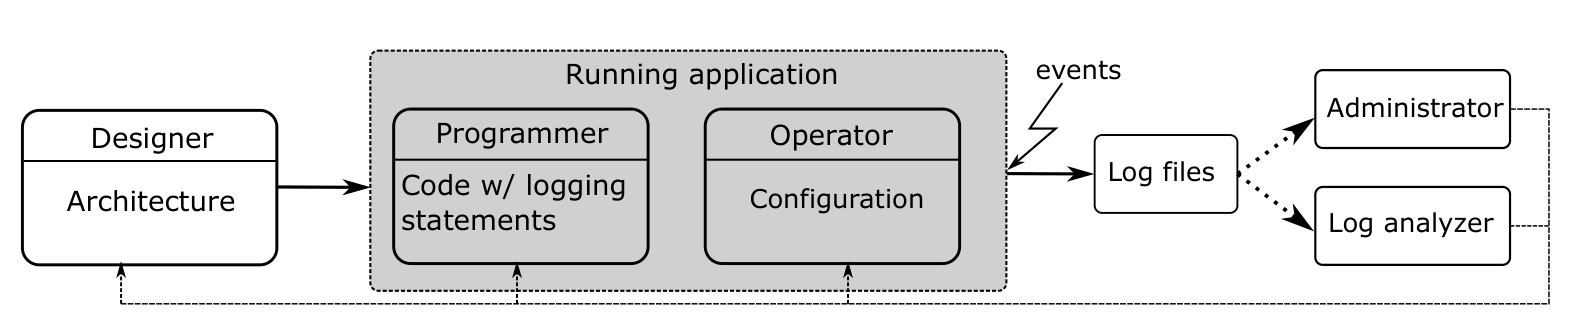
\includegraphics[keepaspectratio=true,scale=0.5]{figures/4_methods/2_log_creation.png}
%    \caption{Framework for creation and analysis of logs. \cite{gholamian2022comprehensive}}
%    \label{fig:logCreation}
%\end{figure}

Log messages often contain contextual information like time stamps, executing program, program version, user and more. Sometimes this information is just noise, sometimes it is critical for tasks such as anomaly detection. 

\subsection{Log File}
\label{sec:Methods:Fundamentals:Logfile}

A log file is a collection of log messages that is persistently stored on a storage medium, also called "event logs", "execution logs" or just "logs". In most cases, these terms are used interchangeably as well and we prefer to use "logs". Modern systems can produce logs in the order of multiple gigabytes per hour, so processing them in an efficient manner is very important \cite{zhu2019tools}. Sometimes these log messages are accompanied by extensive metadata and organised in a more structured manner, sometimes they are just the output to stdout from a system and need to be manually organised. 

\subsection{Log Parsing}
\label{sec:Methods:Fundamentals:Parsing}

Log parsing is a crucial process in the field of log analysis, where the primary objective is to extract structured information from unstructured or semi-structured log data. Logs, generated by various systems and applications, often contain valuable information about the system's state, performance, and potential issues. However, this information is typically embedded in textual log messages that can be difficult to process and analyze due to their unstructured nature and the sheer volume of data.\\

The idea of log parsing is to approximate how a given log line is produced in the source code. The log parsing process involves applying algorithms to identify recurring patterns and variable parts within log messages. By recognizing these patterns, log parsing algorithms can extract the essential components of each log message and represent them in a structured format. This structured representation, often in the form of log templates, simplifies the log data and makes it more accessible for further analysis. Traditionally, this log parsing has been done with regular expressions, but nowadays logging code can update on the scale of thousands of log statements per month in a big organisation, so keeping up with regular expressions is impossible \cite{zhu2019tools}.\\

Log parsing typically serves as the first step towards downstream log analysis tasks. Parsing textual log messages into a structured format enables efficient search, filtering, grouping, counting, and sophisticated mining of logs. The parsed logs can be used in numerous application domains, including but not limited to:

\begin{enumerate}
    \item  Anomaly Detection: By extracting structured information from log data, log parsing facilitates the identification of unusual patterns or behaviors that may indicate system faults or security breaches.
    \item Root Cause Analysis: The extracted information can be used to trace the origin of system failures or performance issues and facilitate timely resolution.
    \item System Performance Monitoring: With structured log data, system administrators and engineers can monitor various performance metrics, identify trends, and optimize system performance.
    \item Security Analysis: Log parsing allows security analysts to detect potential threats, intrusions, or vulnerabilities in a system by analyzing structured log data for suspicious activities or patterns.
\end{enumerate}
Through this log parsing step, log data can be treated as categorical input data to a machine learning model rather than unstructured textual data.

\subsection{Log Templates}
\label{sec:Methods:Fundamentals:Templates}
A log template is a simplified representation of a log message, containing fixed patterns and placeholders for variable parts. The fixed patterns represent the common structure shared by a group of log messages, while the placeholders capture the variable information specific to individual messages. For example, a log template might look like this: "User <*> logged in at <*>", where <*> is a placeholder for the variable parts, in this case User ID and time stamp \cite{zhu2019tools}. \\

Different algorithms employ various techniques to create templates, such as clustering, pattern mining or longest common sub sequence. This way, they effectively reduce the complexity of the log data. The number of templates generated depends on the algorithm and its parameters and ranges between finer/more templates (less substitutions) and coarser/less templates (more substitutions). \\

Using log templates offers several benefits, including improved readability, reduced storage requirements, and faster processing times. However, generating log templates can be challenging due to noisy or inconsistent log messages, determining the optimal granularity of templates, and selecting suitable algorithms and parameters.


% PAWEL: Ich würde dieses Beispiel und die Grafik gerne übernehmen und drin lassen, da es explizit HDFS zeigt was wir benutzen und ich es weiter unten referenzieren kann wenn ich darüber spreche, welche Attribute wir für die prediction benutzen. 
\begin{figure}[H]
    \centering
    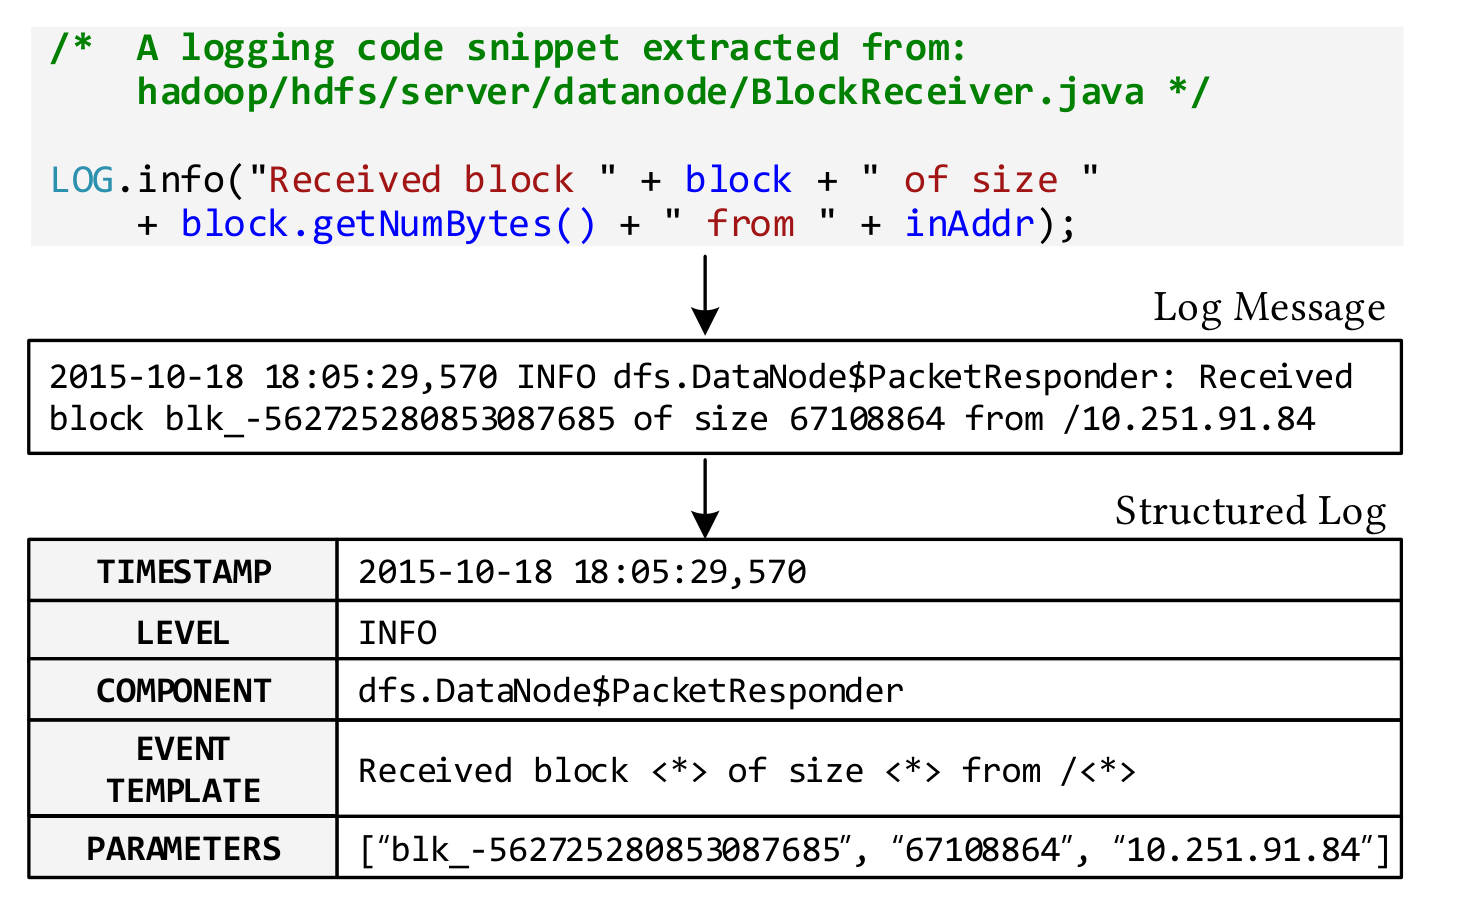
\includegraphics[keepaspectratio=true,scale=0.5]{figures/4_methods/1_log_template_generation.png}
    \caption{An illustrative example of log parsing and log templates \cite{zhu2019tools}.}
    \label{fig:logTemplateGeneration}
\end{figure}
 

\subsection{Text Log Analysis Process}
\label{sec:Methods:Fundamentals:Analysis}
In the current industry standard text log analysis process, administrators face the challenge of selecting an appropriate log parsing algorithm and parameterization that best suits their specific log data. This process typically involves the following steps:

\begin{enumerate}
    \item    Research: Administrators begin by investigating various log parsing algorithms available in the literature or through open-source tools. They must consider the strengths and weaknesses of each algorithm, as well as their suitability for the specific log data they will be analyzing.

    \item    Preliminary Testing: With a selection of candidate algorithms, administrators may conduct a series of limited tests on a small subset of their log data. These tests often involve experimenting with different parameterizations to gauge the performance of each algorithm.

    \item  Algorithm Selection: Based on the results of the preliminary tests, administrators choose the algorithm and parameterization that demonstrated the best performance on their specific log data. This decision is typically made using a combination of quantitative metrics, such as accuracy and efficiency, and qualitative factors, such as ease of implementation and maintainability.

    \item  Fixed Deployment: Once an algorithm and parameterization have been selected, administrators deploy the chosen solution for all future log analysis tasks. This fixed deployment approach assumes that the chosen algorithm and parameterization will continue to perform well on new log data, despite potential changes in log structure or system behavior.
\end{enumerate}
This industry standard process, while practical and widely adopted, has certain limitations. Relying on a fixed algorithm and parameterization may lead to sub optimal results, as it does not account for variations in log data or evolving system requirements. Furthermore, administrators may not have the time or expertise to thoroughly test and compare all available algorithms and parameterizations, potentially leading to the selection of a sub optimal solution.\\

In this context, the development of an automated method for selecting log parsing algorithms and parameterizations, such as the attention-based approach proposed in this thesis, holds significant potential for improving the efficiency and effectiveness of the text log analysis process. By dynamically adapting to the specific log data and analysis task at hand, such a method can help address the limitations of the current industry standard process and contribute to the advancement of log analysis techniques.\\

Figure \ref{fig:process} shows the current log analysis process. Raw logs are produced by the system in a format that can not be utilized for machine learning tasks. A parsing algorithm takes these kind of log messages and converts them into a log template by identifying fixed (highlighted in blue) vs variable (highlighted in yellow) parts. These templates are then used to train a machine learning model for prediction tasks such as next template prediction. 
\begin{figure}[H]
    \centering
    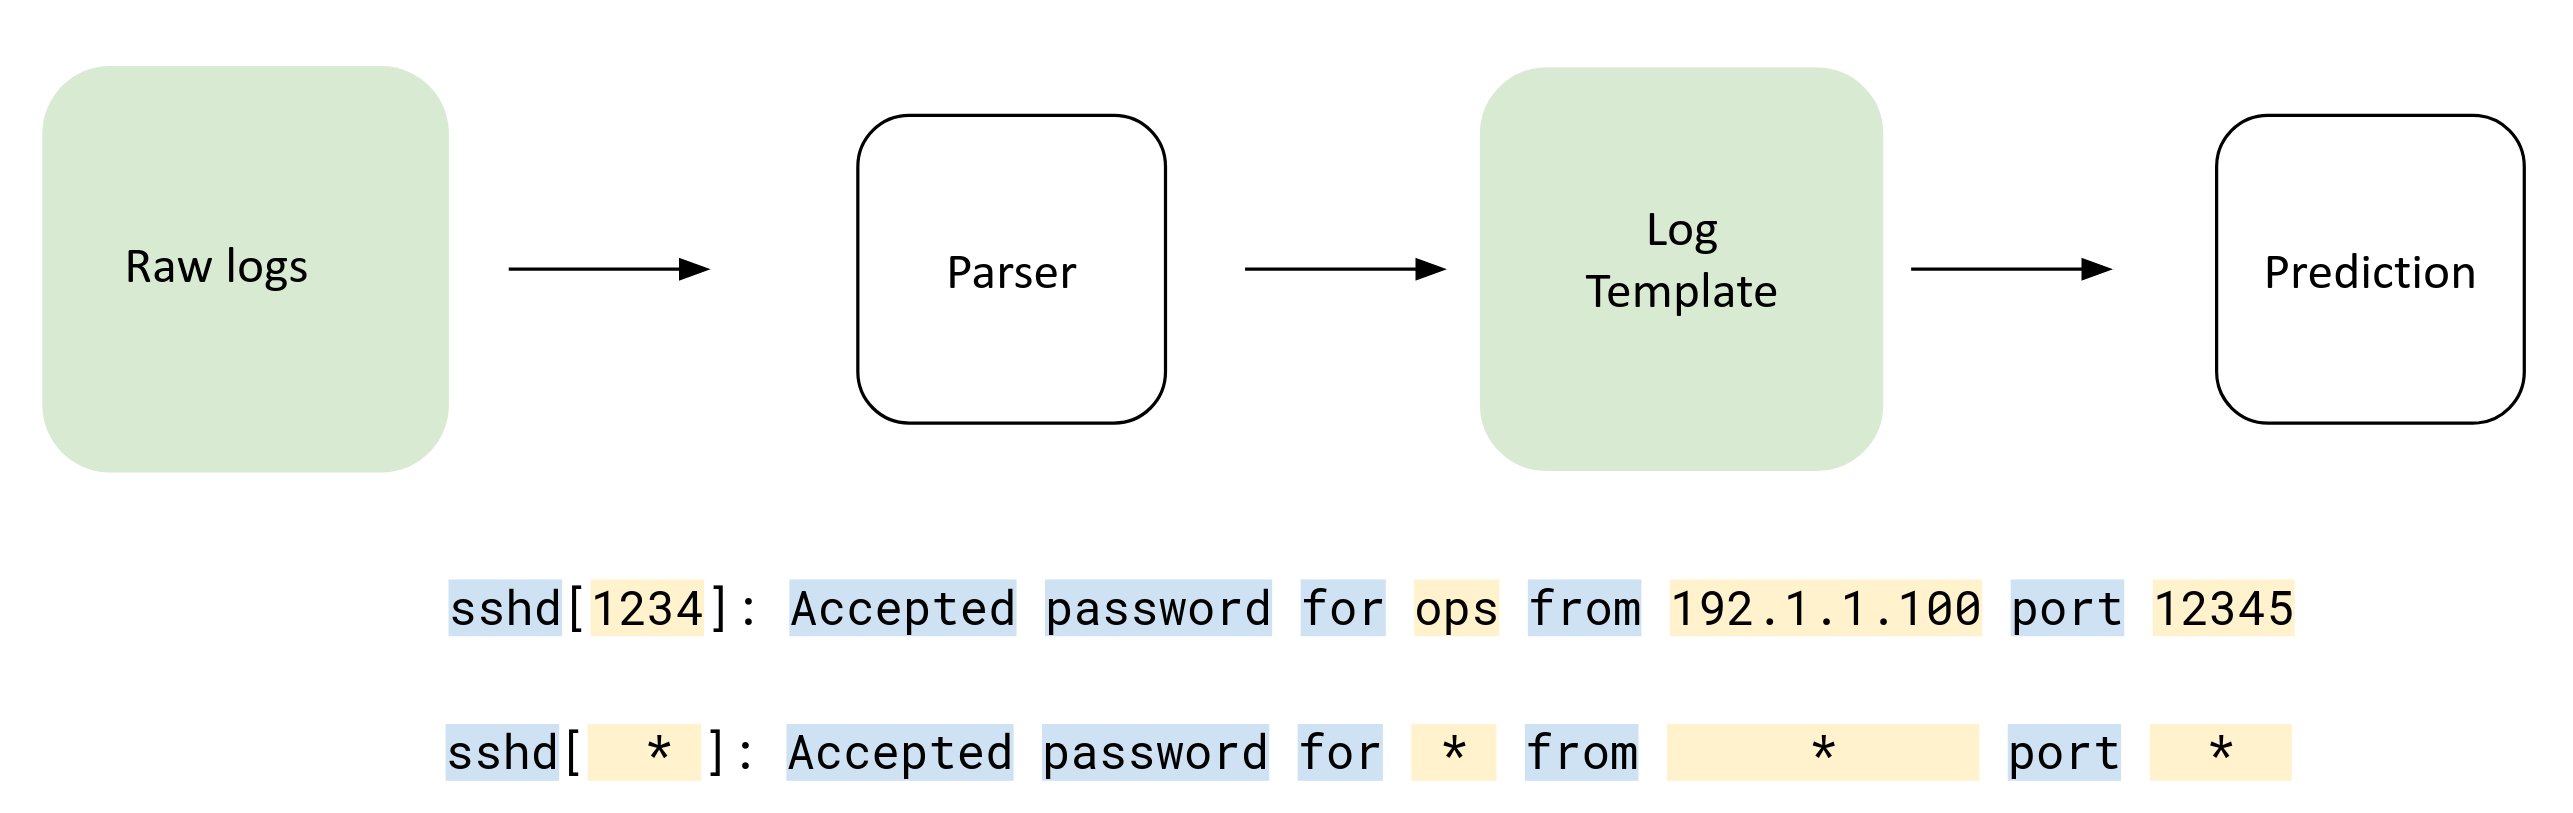
\includegraphics[keepaspectratio=true,scale=0.3]{figures/4_methods/3_text_log_analysis_process.png}
    \caption{The current industry standard text log analysis process}
    \label{fig:process}
\end{figure}

\subsection{Attention Mechanism and prediction model}
\label{sec:Methods:Fundamentals:Attention}
The attention mechanism has its origins in natural  language processing \cite{bahdanau2016neural} and has since been successfully applied to various tasks in machine learning and artificial intelligence. Attention mechanisms were first introduced by Bahdanau et al. in the context of neural machine translation, where they were used to improve the alignment between input and output sequences by allowing the model to focus on different parts of the input sequence during the generation of each output element. At its core, the attention mechanism computes a weighted sum of input elements, where the weights represent the relevance or "attention" paid to each element.\\

This attention mechanism has been further developed for healthcare prediction by Choi et al \cite{choi2017gram}. They call their improved method "graph based attention", because it leverages a knowledge graph that is combined with the input and fed into the attention mechanism. The knowledge graph (symptom hierarchy) and input (symptoms per visit) are used to calculate attention embeddings, which are trained together with the model on the task of next symptom prediction. 
Figure \ref{fig:healthcare} shows the overall structure of healthcare prediction with graph based attention which we then adapt in \ref{fig:monitoring} for our log analysis task. \\

The knowledge graph in healthcare is based on ICD-9 codes, which model a hierarchy of symptoms and diseases and utilizes domain knowledge crafted by medical experts over several decades. An example can be seen in \ref{fig:icd9}.
\begin{figure}[H]
    \centering
    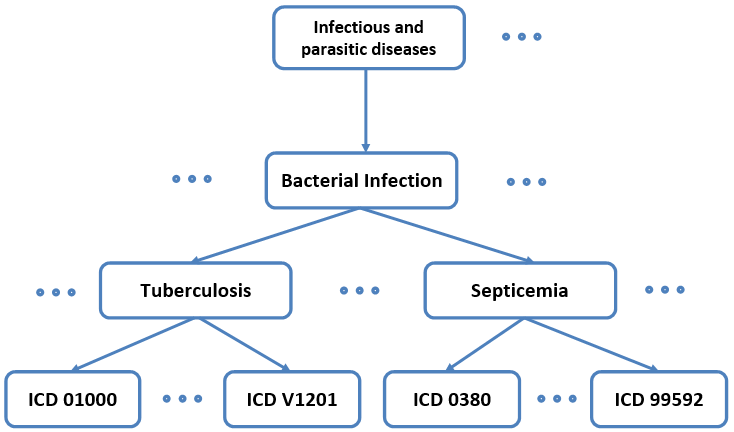
\includegraphics[keepaspectratio=true,scale=0.3]{figures/4_methods/ICD-9-hierarchy-of-diseases.png}
    \caption{Example hierarchical knowledge graph based on ICD-9 codes \cite{icd9}.}
    \label{fig:icd9}
\end{figure}

\begin{figure}[H]
    \centering
    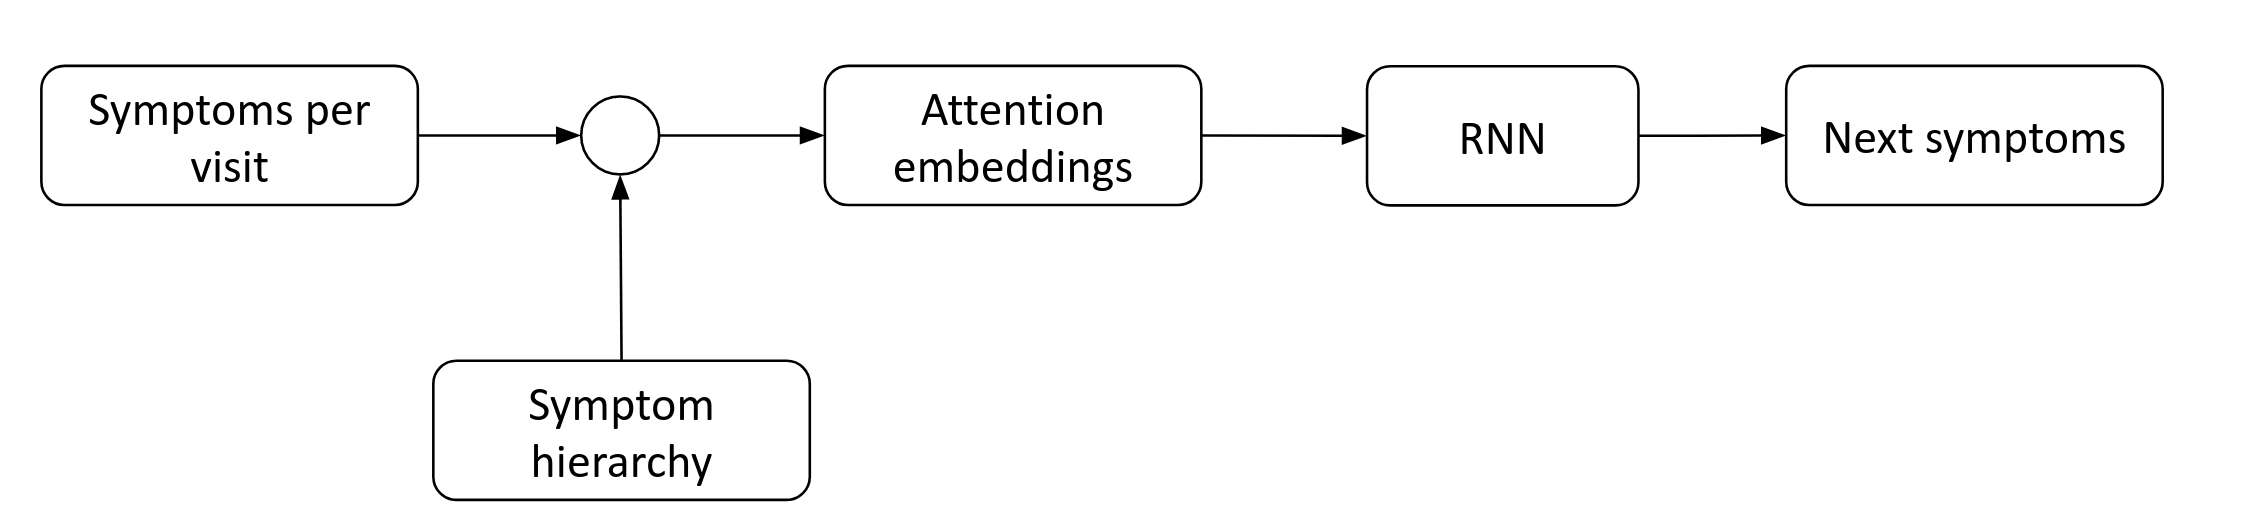
\includegraphics[keepaspectratio=true,scale=0.3]{figures/4_methods/8_healthcare.png}
    \caption{The structure of healthcare prediction using gram \cite{choi2017gram}}.
    \label{fig:healthcare}
\end{figure}

\begin{figure}[H]
    \centering
    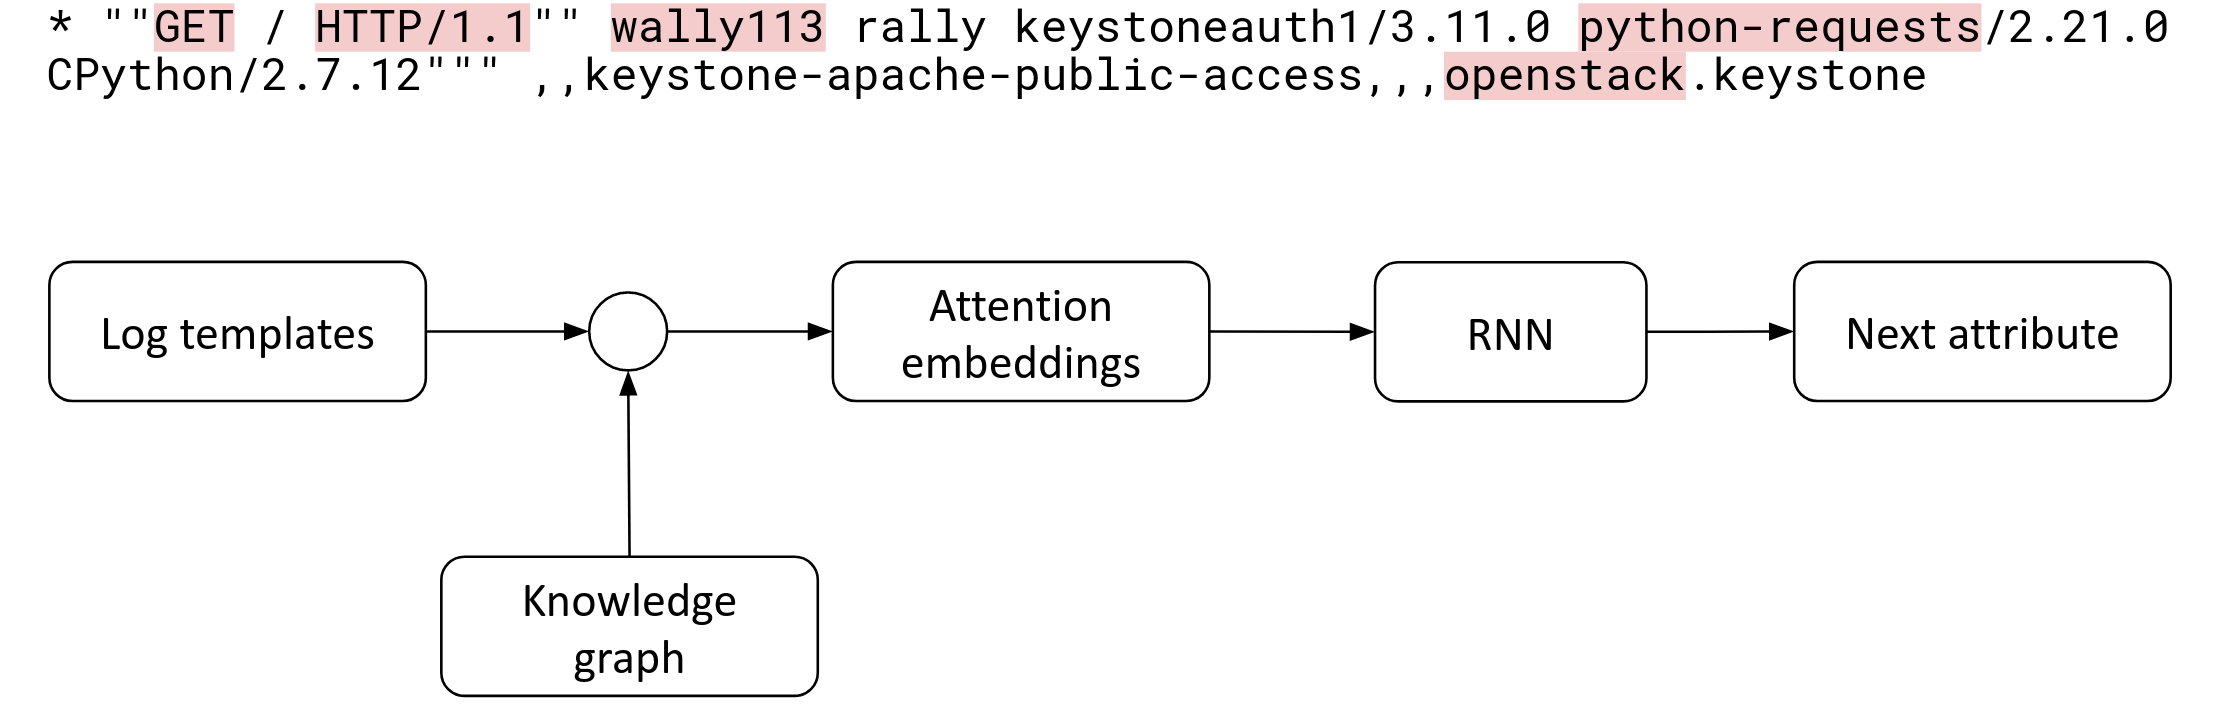
\includegraphics[keepaspectratio=true,scale=0.3]{figures/4_methods/9_monitoring.png}
    \caption{Our attention based log template selection. Highlighted in red are the attributes for next attribute prediction.}
    \label{fig:monitoring}
\end{figure}

In healthcare, we calculate attention weights by first computing similarity scores between a leaf in the knowledge graph and all of its ancestors using a softmax function and a feed forward neural network with a single hidden layer. After calculating the individual attention weights, we multiply them with the base embeddings of each of our nodes and then sum the results up to get a final attention embedding for the leaf node. This is done to give more importance to diseases that are more rare in the dataset. Figure \ref{fig:gramAttention} visualises the computation of the attention weights for covid between its ancestors. 

\begin{figure}[H]
    \centering
    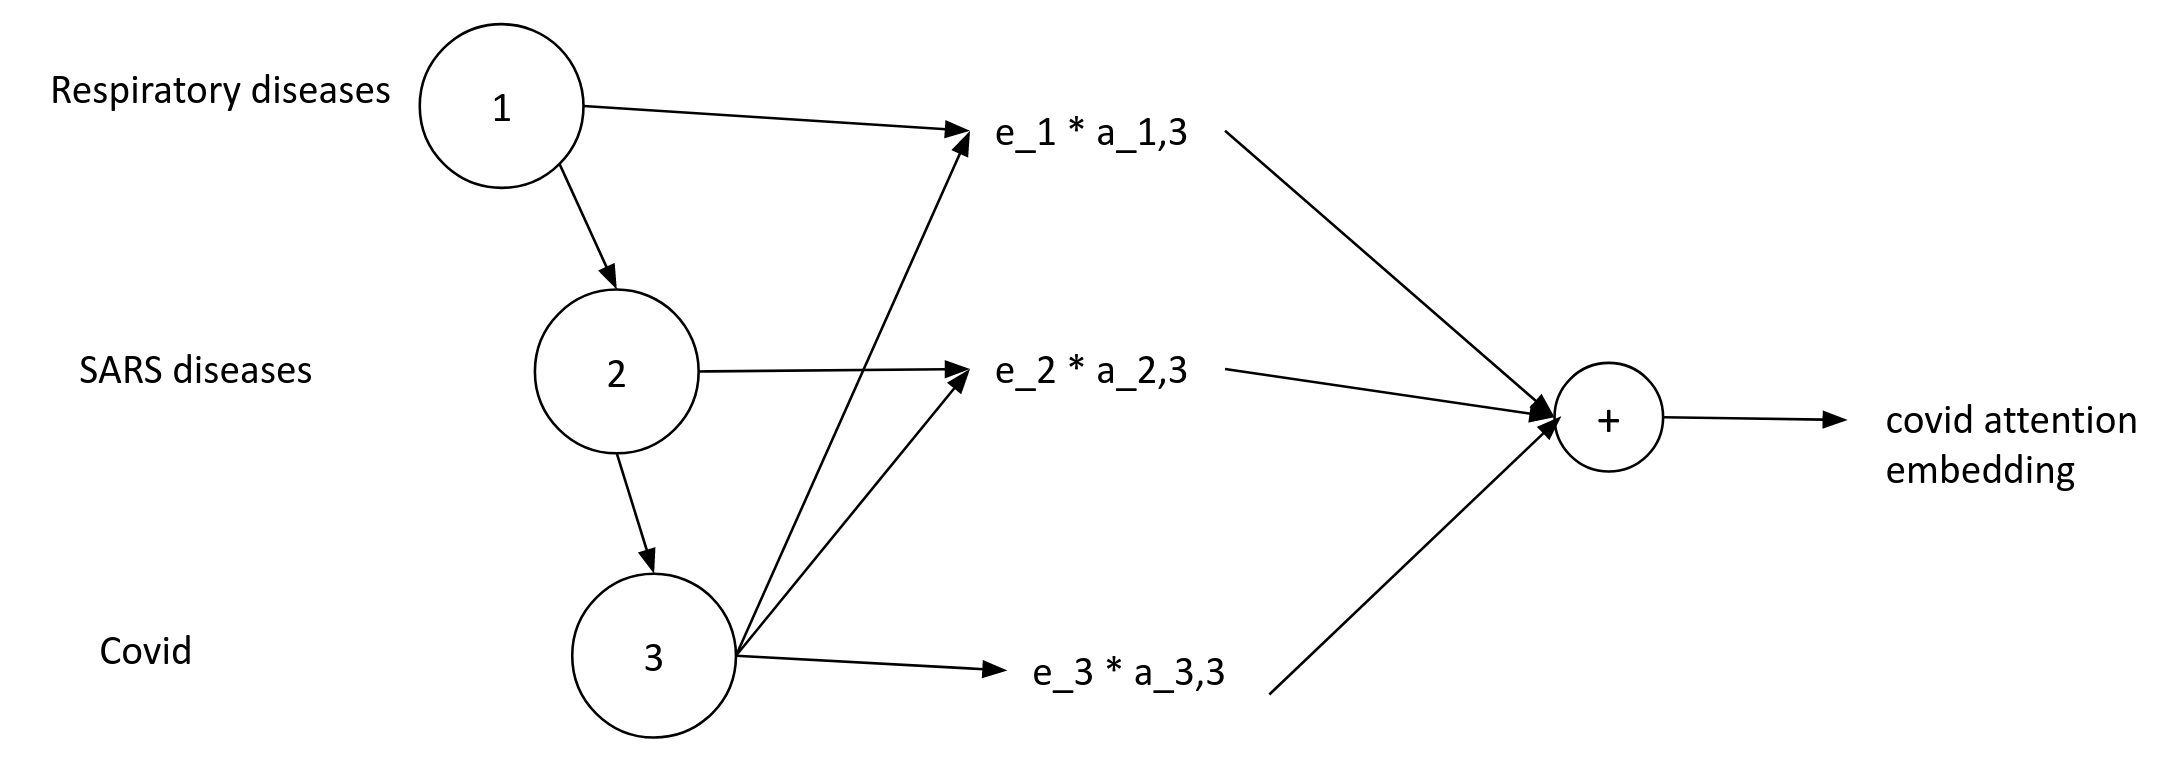
\includegraphics[keepaspectratio=true,scale=0.3]{sections/gram_attention.png}
    \caption{Computation of attention weights with gram for healthcare. }
    \label{fig:gramAttention}
\end{figure}

For our log analysis task, we utilize softmax and feed forward neural network as well, but instead of calculating the attention weights between leafs and ancestors, we calculate them for each node and its neighbors. 

\begin{figure}[H]
    \centering
    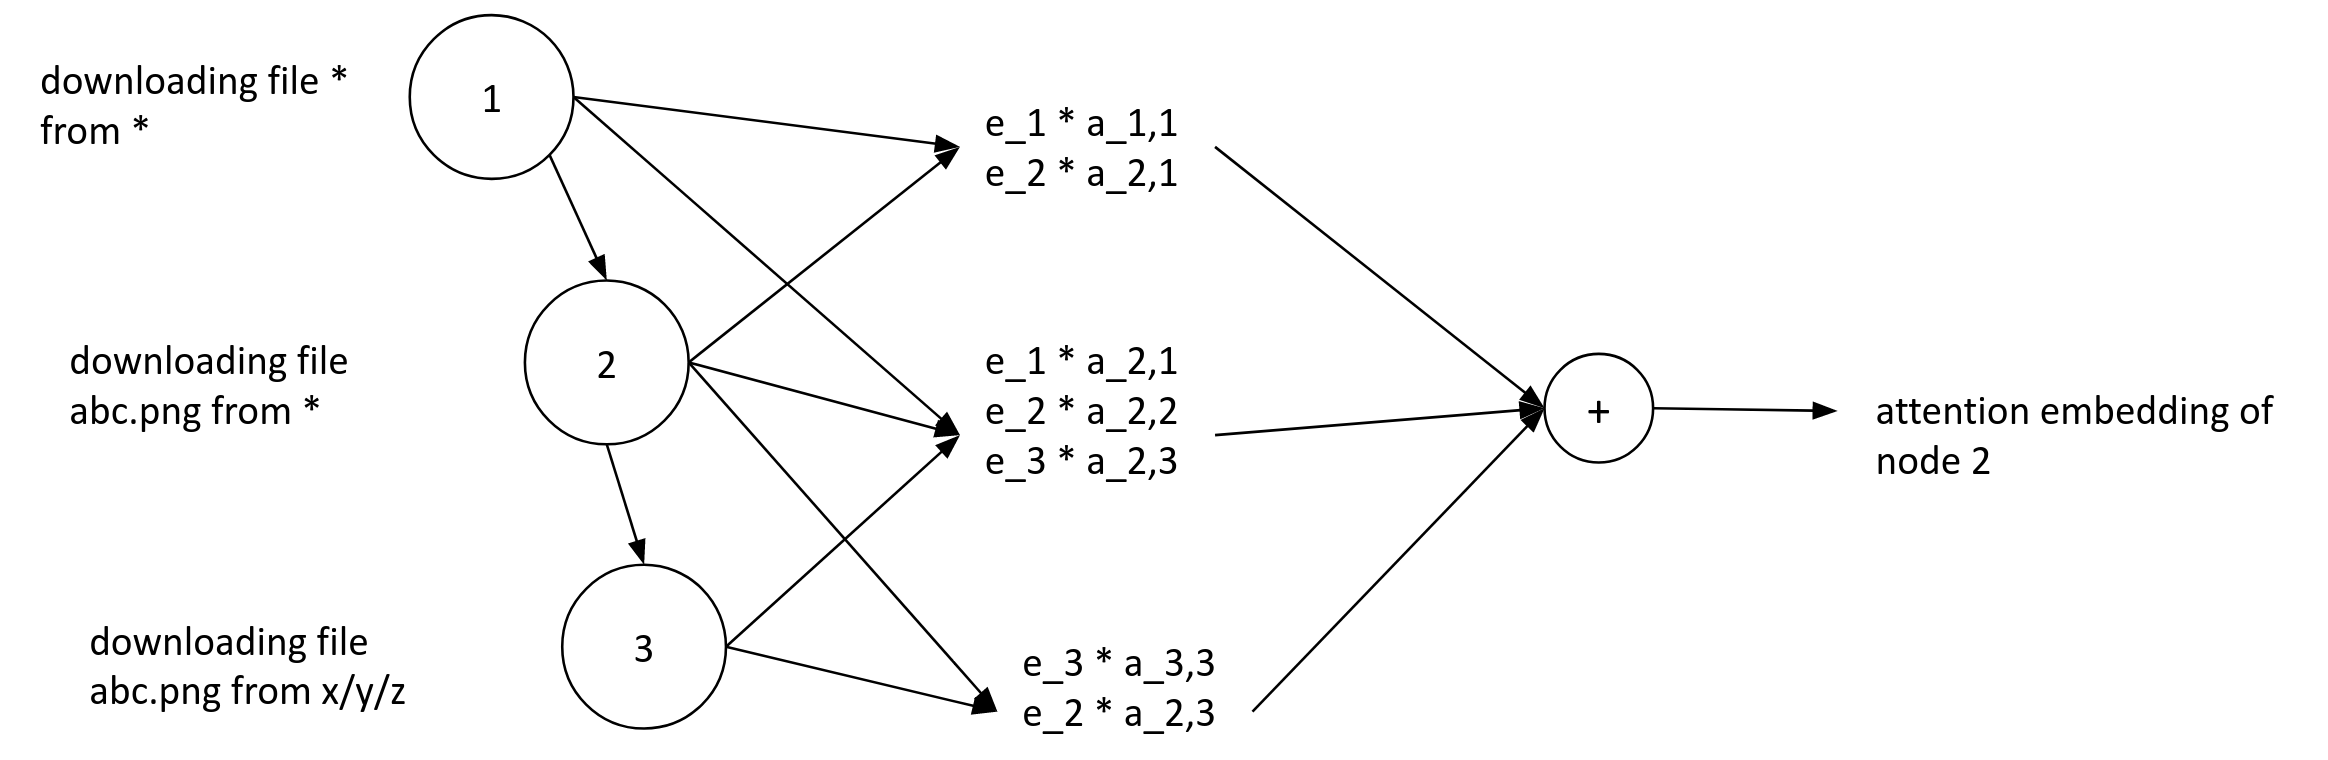
\includegraphics[keepaspectratio=true,scale=0.3]{figures/4_methods/log_attention.png}
    \caption{Computation of attention weights with gram for log analysis.}
    \label{fig:gramAttentionLogs}
\end{figure}

The general equation to calculate the attention embeddings is as follows, where $v_j$ are the nodes in the connected features $C_i$ and $a_{i,j}$ are the attention weights between the nodes $i$ and $j$ calculated by softmax and $e_j^b$ are the base embeddings for node $j$. 

\begin{equation}
    e_i^a=\sum_{v_j \in C_i \cup\left\{v_i\right\}} \alpha_{i, j} e_j^b \in \mathbb{R}^{\operatorname{dim}_e}
\end{equation}

\section{Log Parsing Algorithms}
\label{sec:Methods:Algorithms}
In the prior Master Thesis \cite{witterauf2021domainml}, the heuristical log parsing algorithm Drain \cite{drain} was used. To test whether the promising method of attention based log template selection also applies to other parsing algorithms, we chose two other well performing algorithms that follow different parsing approaches, namely Spell \cite{spell} and Nulog \cite{nedelkoski2020selfsupervised}. All three of these have been evaluated on the datasets provided by \cite{zhu2019tools} and performed very well. All of them process logs in a streaming manner, meaning that they can  parse log messages as they are generated, without waiting for the whole log file to be available. This way, the log parser can provide real-time analysis and monitoring of the system behavior. \\

The Tools and Benchmarks for Automated Log Parsing paper \cite{zhu2019tools} provides an extensive framework to evaluate the performance of log parsers on 16 different datasets. They also provide their own, uniform, implementation of each log parser. The additional datasets that we have chosen for this work have been taken from their paper. \\

The parameters that we have chosen for each algorithm stay the same for all datasets, to avoid introducing additional variability. They are most certainly not chosen optimally, but for our work this is ideal since it reflects the use case we try to improve.

\subsection{Drain}
\label{sec:Methods:Algorithms:Drain}

Drain, which stands for depth tree based online log parsing \cite{drain}, is a widely used log parsing algorithm known for its efficiency and effectiveness in extracting structured information from unstructured or semi-structured log data. Drain employs a heuristic-based approach, which enables it to efficiently group similar log messages and generate log templates that capture the underlying patterns in the data. It consists of multiple steps but starts by
preprocessing the log messages using regex rules that are dependent on the dataset and defined by the administrator based on domain knowledge.
Afterwards, the log text is split into a list of words. These are then used to build the parse tree.
This tree has a fixed size, which is defined by the parameter Depth and avoids
constructing a deep and unbalanced tree \cite{drain}. The difficulty with drain is to find good parameters for the dataset. Once these are found, it performs better than most other log parsing algorithms in the benchmarks \cite{zhu2019tools}. \\

Key features of the Drain algorithm include:

\begin{enumerate}
    \item  \textbf{Incremental processing}: Drain processes log messages incrementally, allowing it to handle large-scale log datasets and adapt to changes in log patterns over time.
    \item  \textbf{Fixed-depth parse tree}: Drain organizes log messages in a fixed-depth parse tree, which significantly reduces the search space and speeds up the clustering process.
    \item  \textbf{Online parsing}: Drain parses logs in a streaming manner, instead of processing batches of log data offline to train a data mining model, enabling it to efficiently group log messages in real-time as they are processed.
    \item  \textbf{Parameterization}: Drain offers two primary parameters, log depth and log similarity threshold, which control the granularity of the generated log templates and can be tuned to optimize the algorithm's performance for specific log analysis tasks.
\end{enumerate}

In our research, Drain is a suitable choice for several reasons:
\begin{enumerate}
    \item \textbf{Scalability}: Drain's incremental processing and efficient clustering approach make it well-suited for handling large-scale log datasets and adapting to changes in log patterns over time, which are common challenges in log analysis.
    \item \textbf{Flexibility}: Drain's parameterization allows us to explore different levels of granularity in the generated log templates, enabling us to investigate the impact of varying parameter settings on the performance of our attention-based method.
    \item \textbf{Comparability}: As a widely used and well-established log parsing algorithm, Drain serves as a useful benchmark for comparing the performance of our attention-based method with existing approaches in the literature.
\end{enumerate}


The implementation for drain that we use stems from \cite{drainrepo}, which unfortunately is not available anymore. 

%TODO: include figure that visualises drain, more explanations of how the tree is built and logs processed?
\begin{table}[h]
\centering
\begin{tabular}{|c|c|c|}
\hline
\textbf{Parameter Setting} & \textbf{Log Depth} & \textbf{Log Similarity Threshold} \\ \hline
Fine Drain   & 10 & 0.75 \\ \hline
Medium Drain & 7  & 0.4  \\ \hline
Coarse Drain & 4  & 0.2  \\ \hline
\end{tabular}
\caption{Drain parameter settings}
\label{table:drain_parameters}
\end{table}

We have taken the coarse and fine settings from the original master thesis \cite{witterauf2021domainml} and expanded with medium drain settings, which are roughly in the middle of their respective range. Note, that these settings were originally chosen for the Huawei dataset, but will also be chosen for the other datasets.  The concrete parameters can be seen in table \ref{table:drain_parameters}. 

\subsection{Spell}
\label{sec:Methods:Algorithms:Spell}
% Should I explain the LCS problem? Appendix?
Spell, which stands for Streaming Parser for Event Logs using an LCS \cite{spell}, is an approach that uses the longest-common sub sequence technique (LCS). The algorithm is available in two versions, the original version from 2016 and an improved, parallelized version from 2019. In this work we use the older, less efficient version, because no public implementation of the improved version is available. We took the implementation from \cite{zhu2019tools} and adapted it for our framework \cite{witterauf2021domainml}.\\

Spell underlies a key assumption: If we view the output by a log printing statement (which is a log entry) as a sequence , in most log printing statements, the constant that represents a log template often takes a majority part of the sequence and the parameter values take only a small portion. If two log entries are produced by the same log printing statement stat , but only differ by having different parameter values, the LCS of the two sequences is very likely to be the constant, implying a message type.\\

Spell is another popular log parsing algorithm that has been widely used for extracting structured information from unstructured or semi-structured log data. It employs a sequential approach that processes log messages one by one, aligning them with existing log templates or creating new templates as needed.\\

Key features of the Spell algorithm include:
\begin{enumerate}
    \item \textbf{Independence of domain knowledge}: contrary to drain needing regular expressions, spell aims to avoid domain knowledge all together
    \item \textbf{Parameterization}: Spell offers a single primary parameter, its threshold, which controls the granularity of the generated log templates and can be tuned to optimize the algorithms's performance for specific log analysis tasks. 
    \item \textbf{Potential for speedup}: with parallelization and the additional parameters split threshold and merge threshold, the performance of spell can be greatly increased. 
\end{enumerate}

% TODO: explain spell steps in more detail
Similar to drain, spell starts by preprocessing the incoming log messages. This step involves tokenization, where each log message is split into a sequence of tokens based on pre-defined delimiters, such as space and equal sign. For each incoming log message, spell compares the message with existing log templates in the template pool. If the incoming log message matches an existing log template with a similarity above the message type threshold, the log message is aligned with that template. If no matching template is found, a new log template is created for the incoming log message.
\begin{figure}[H]
    \centering
    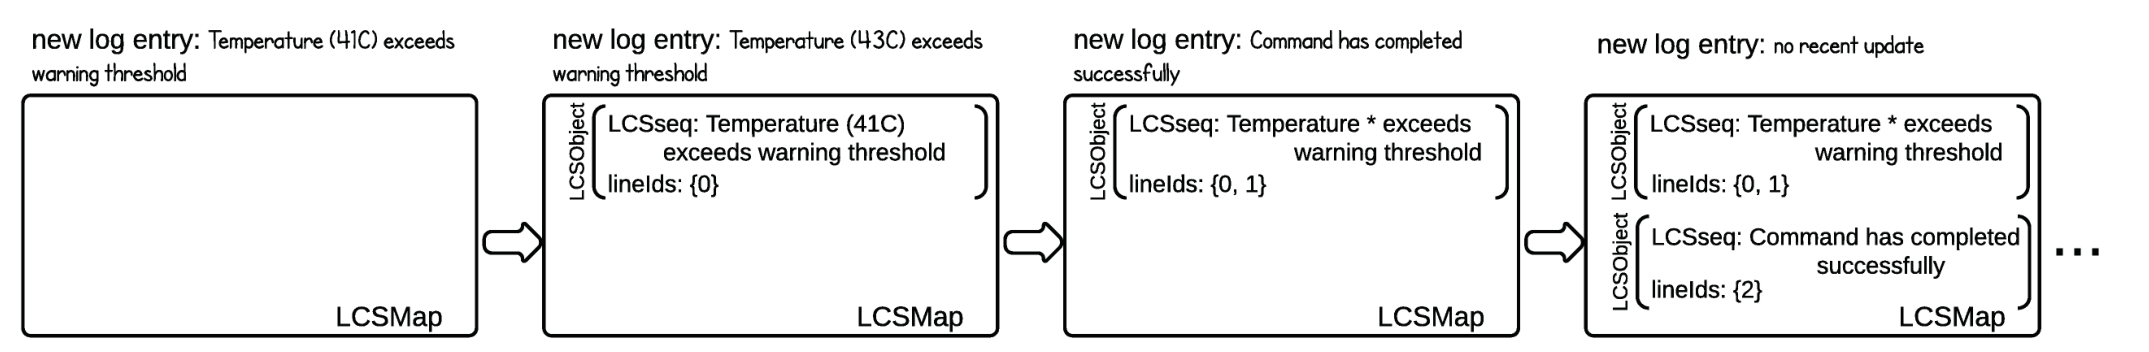
\includegraphics[keepaspectratio=true,scale=0.45]{figures/4_methods/5_spell_workflow.png}
    \caption{Basic Spell workflow \cite{spell}.}
    \label{fig:spellWorkflow}
\end{figure}

For the threshold parameter we selected values between 0.5 and 0.9, because in our tests 0.5 already produced the coarsest templates and there was no benefit of choosing a lower value. As with drain, these values are chosen identically for all datasets that we run our experiments on. 

\begin{table}[h]
\centering
\begin{tabular}{|c|c|}
\hline
\textbf{Parameter Setting} & \textbf{Message Type Threshold} \\ \hline
Fine Spell   & 0.9 \\ \hline
Medium Spell & 0.7 \\ \hline
Coarse Spell & 0.5 \\ \hline
\end{tabular}
\caption{Threshold parameters for Spell}
\label{tab:spell_parameters}
\end{table}

\subsection{NuLog}
\label{sec:Methods:Algorithms:NuLog}

NuLog is a state-of-the-art log parsing algorithm that leverages neural parsing techniques to extract structured information from unstructured or semi-structured log data \cite{nedelkoski2020selfsupervised}. Unlike traditional rule-based or clustering-based approaches, NuLog formulates the log parsing task as a masked language modeling (MLM) problem and employs self-supervised learning to train the model. By leveraging self-supervised learning, NuLog can effectively learn from the log data without requiring explicit supervision in the form of labeled data. This makes the algorithm more scalable and applicable to a wide range of log datasets.\\


The NuLog algorithm consists of three main steps:
\begin{enumerate}
    \item \textbf{Preprocessing}: Each log message is split into tokens, and a percentage of tokens are replaced by masking tokens. This step prepares the log data for the subsequent masked language modeling task.
    \item \textbf{Model training}: A transformer-based neural network is trained to predict the masked tokens in the log messages. During training, the model learns to capture the structure and patterns in the log data.
    \item \textbf{Template extraction}: Based on the predictions made by the neural network model, a vector representation of the log messages is generated. Using this representation, NuLog extracts log templates that capture the underlying structure of the log data.
\end{enumerate}

\begin{figure}[H]
    \centering
    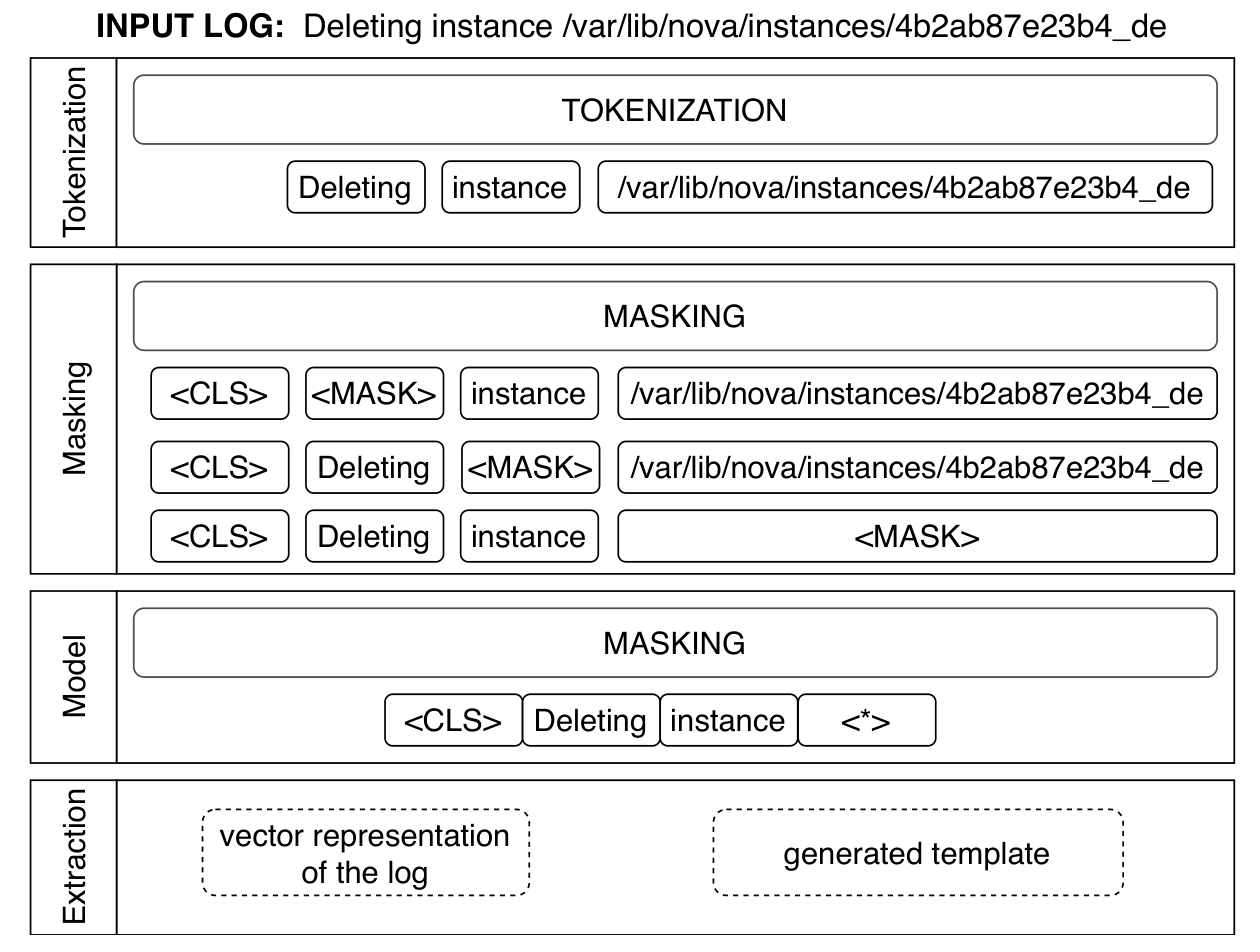
\includegraphics[keepaspectratio=true,scale=0.55]{figures/4_methods/6_nulog_workflow.png}
    \caption{Instance of parsing of a single log message with NuLog \cite{nedelkoski2020selfsupervised}.}
    \label{fig:nulogWorkflow}
\end{figure}

One of the main strengths of NuLog is its robustness across various environments and log data types. Due to its neural parsing approach, NuLog can effectively adapt to diverse log patterns, making it a suitable choice for log analysis tasks in different domains and systems. A big downside is its runtime, being orders of magnitude slower than drain and spell. \\

The following figure shows a benchmark that illustrates the superiority of NuLog in terms of robustness. The figure shows the accuracy distribution of each log parser across the log datasets provided in \cite{zhu2019tools}. We can see that the parsers selected by us are the three top performing ones. 

\begin{figure}[H]
    \centering
    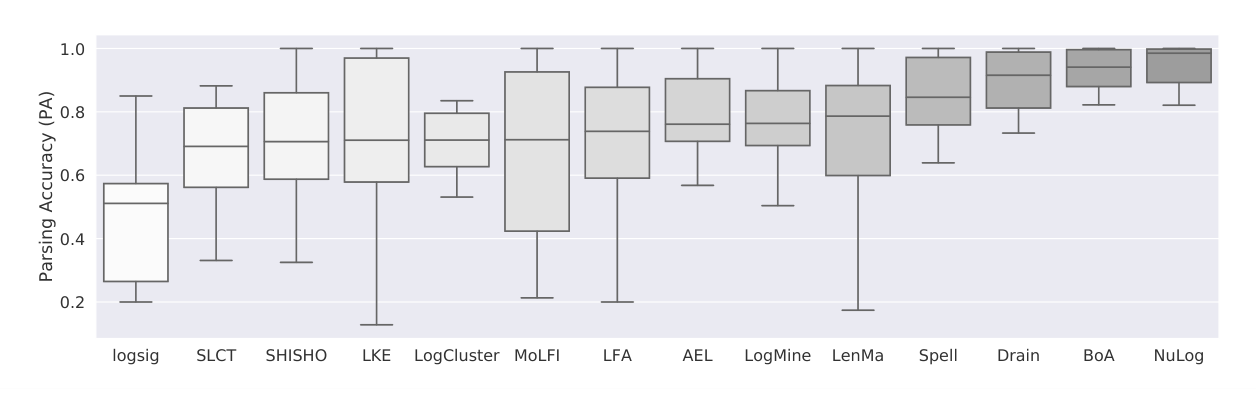
\includegraphics[keepaspectratio=true,scale=0.7]{figures/4_methods/7_parser_accuracy_robustness.png}
    \caption{ Robustness evaluation on the parsing accuracy of the log parsers \cite{nedelkoski2020selfsupervised}.}
    \label{fig:parserAccuracy}
\end{figure}

NuLog can be controlled by manipulating a parameter $k$, which the index of each element in the positional vector $p$. It describes an exponential relationship between each value of the vector $p$ in the following equation, where $j$ is the positional index of each token:
\begin{equation}
p_{2 k}=\sin \left(\frac{j}{10000^{\frac{2 k}{v}}}\right), p_{2 k+1}=\cos \left(\frac{j}{10000^{\frac{2 k+1}{v}}}\right)
\end{equation}
For the selection of this parameter, we have taken inspiration from the parameters that the NuLog authors chose when performing the benchmarks from \cite{zhu2019tools}. We selected the highest value chosen by them as our "coarse" value and the lowest value as our "fine". It was not immediately apparent how the variation of this parameter affects the template generation, so we stuck with the naming scheme for the sake of unity. \\

\begin{table}[h]
\centering
\begin{tabular}{|c|c|}
\hline
\textbf{Parameter Setting} & \textbf{Parameter $k$} \\ \hline
Fine NuLog   & 5  \\ \hline
Medium NuLog & 20 \\ \hline
Coarse NuLog & 50 \\ \hline
\end{tabular}
\caption{Parameter settings for NuLog}
\label{tab:nulog_parameters}
\end{table}


\section{Datasets}
\label{sec:Methods:Datasets}
In this work, we build upon the dataset utilized in the preceding master's thesis that serves as the foundation for our work. To ensure diversity in our analysis, we have incorporated two additional datasets, which were previously employed in the tools and benchmarks paper \cite{zhu2019tools}. These datasets exhibit distinct characteristics compared to our initial dataset, making them a valuable addition to our research.\\

The log parsing algorithms have been evaluated on these supplementary datasets, and their respective implementations have been provided by the same authors who contributed the datasets. This ensures a seamless integration of the algorithms with the datasets, enhancing the reliability of our experiments.\\

It is important to note that while the complete Huawei dataset was used in the original master's thesis, we have opted to limit our analysis to a subset of 2,000 log messages due to the slower performance of other algorithms. This decision aligns our study with the tools and bechmarks and the NuLog paper, both of which also evaluated their algorithms on 2,000 log messages, thereby facilitating a more accurate comparison between our work and these studies.

\subsection{Huawei Logs}
\label{sec:Methods:Datasets:Huawei}
This dataset, originating from the study by \cite{10.1007/978-3-030-44769-4_13}, was specifically designed to facilitate research in the realm of multi-source, AI-driven analytics. The dataset encompasses logs, metrics, and traces; however, for the purposes of this study, only the logs and the concurrent setting are utilized. The log messages possess 23 attributes, but only eight are relevant to the prediction task and used to train our model. These include:

\begin{enumerate}
    \item Hostname
    \item log\_level
    \item programname
    \item python\_module
    \item http\_status
    \item http\_method
    \item Payload
    \item http\_url 
\end{enumerate}

Originally, the master thesis also used timestamps, but we found them out to be noise and removed them. More on that in a later section. 

\begin{table}[h]
\centering
\begin{tabular}{c|c}
\hline Number of log lines & 169230 \\
Number of log templates & 1446 \\
Number of log attributes & 176 \\
Avg. number of attributes per log & 4.2 \\
Max. number of attributes per log & 5 \\
\hline
\end{tabular}
\caption{Number of log templates and attributes \cite{witterauf2021domainml}}
\label{tab:logTemplates}
\end{table}

\begin{table}[h]
    \centering
\begin{tabular}{l|ll}
\hline Log Attribute Type & Number of Attributes & Example Attribute \\
\hline Hostname & 5 & wally113 \\
Log Level & 3 & info \\
Programname & 24 & cinder-scheduler \\
Modulename & 95 & cinder.scheduler.host\_manager \\
Endpoint & 34 & auth/login/ \\
HTTP Method & 4 & post \\
HTTP Status & 11 & 404 \\
\hline
\end{tabular}
    \caption{Log Attributes}
    \label{tab:logAttributes}
\end{table}



\subsection{Thunderbird Logs}
\label{sec:Methods:Datasets:Thunderbird}
Thunderbird is an open dataset of logs collected from a Thunderbird supercomputer system. The data has been collected for 244 days and encompasses over 200 million log messages and having a total size of 29.60GB. For our experiments we use a sample log containing 2000 log messages, available under \cite{thunderbirdSampleLogs}. \\

The dataset has five different features, of which we only identify one as relevant for our NAP task: AdminAddr, because the other attributes are only datetime information. The data is also labelled, so it could be used for anomaly detection tasks.\\

In the collection of datasets utilized for this study, the Thunderbird logs exhibit the lowest degree of diversity, characterized by a high level of repetition because of the number of clusters and an abundance of noisy data, predominantly consisting of timestamps and date-related information. The attribute that we want to predict would be dn228/dn228 in the example log below.
\begin{verbatim}
- dn228/dn228 crond(pam_unix)[2915]: session closed for user root
\end{verbatim}

\subsection{HDFS Logs}
\label{sec:Methods:Datasets:HDFS}
HDFS stands for hadoop distributed file system log. The data has been collected over 38.7 hours and contains over eleven million log messages. The datasize is 1.47GB. As with the Thunderbird logs, we use a random sample of 2000 log messages.\\

The dataset has six different features, of which we use all except the datetime information for training and three attributes as prediction targets, namely loglevel, component and Pid (if available), as can be taken from the structured log shown in \ref{fig:logTemplateGeneration}.

\begin{verbatim}
 INFO dfs.DataNode$PacketResponder: PacketResponder 1 for block * terminating
\end{verbatim}
\section{Timestamps}
\label{sec:Methods:Timestamps}
During the course of this thesis, an interesting observation emerged regarding the role of time stamps in log messages. Although not the primary focus of this work, it was deemed worthwhile to explore this aspect further due to its potential impact on next sequence prediction.\\

Time stamps are a common feature in log messages, providing valuable information about the chronological order of events. However, they may also introduce noise, particularly when the data size increases. To investigate this hypothesis, we conducted a series of experiments using the Huawei dataset with and without time stamps.\\

We started by preprocessing the Huawei dataset to remove time stamps from the log messages. We then created several subsets of the dataset with varying sizes to examine the effect of data size on the role of time stamps. The experiments were conducted on these subsets, both with and without time stamps, to assess their impact on next sequence prediction performance. The log parsing algorithm that we used for these experiments was drain. 

\section{Next Sequence Prediction}
\label{sec:Methods:NSP}
Next sequence prediction is a common task in machine learning, where the goal is to predict the subsequent element or sequence of elements in a given dataset based on the previously observed data. This task is often used as a pseudo task, meaning that it serves as a proxy for solving a more complex or less well-defined problem. In such cases, the performance of a model on the next sequence prediction task can provide insights into the model's ability to solve the underlying problem of interest.\\

One prominent application of next sequence prediction as a pseudo task is in anomaly detection \cite{nedelkoski2020selfsupervised}. Anomaly detection involves identifying patterns or data points that deviate significantly from the expected behavior, which can be indicative of errors, faults, or malicious activities. In this context, next sequence prediction can be used as a proxy task to model the normal behavior of a system. By training a model to predict the next sequence of events in a log, for example, we can capture the typical patterns and relationships within the data. Once the model is trained, it can be used to identify deviations from these patterns, which may signal anomalies.\\

In our experiments, we use a derivation of next sequence prediction, which we call "next attribute prediction". Instead of predicting the next log template, we predict the attributes associated with. These attributes are listed in \ref{sec:Methods:Datasets:Huawei} in the case of the Huawei logs.
\section{DomainML}
\label{sec:Methods:DomainML}
This work builds upon an earlier work called DomainML, which was developed by a master student to evaluate the impact of domain knowledge on different data science tasks. We use and enhance the existing DomainML codebase by implementing and incorporating our different log parsing algorithms. DomainML used the attention mechanism in combination with various types of domain knowledge, which we leave out to investigate the sole influence of the attention based selection. 

\section{Experimental Setup and Evaluation}
\label{sec:Methods:Experiments}

In this section, we describe the methodology used to implement the attention-based selection of log templates for automatic log analysis. We build upon the existing framework established in DomainML \cite{witterauf2021domainml} and modify the log parsing step to accommodate the attention mechanism. Our approach consists of the following steps:

\paragraph{Modification of the Log Parsing Step}
The original DomainML framework used two log templates. We expanded this to three log templates with varying levels of granularity. We then implemented two additional log parsing algorithms, taking the total number of parsers to three. The new parsers were integrated into the framework, extending the original one.

\paragraph{Creation of Log Templates}
We executed all three parsers sequentially, allowing each parser to create three log templates. This resulted in a total of nine log templates generated by the three parsers. We also experimented with the different combinations of parsers, namely:
\begin{enumerate}
    \item Spell + NuLog
    \item Spell + Drain
    \item Drain + NuLog
\end{enumerate}


We investigated the performance and quality changes between these combinations to understand the impact of the attention mechanism on log parsing.


\paragraph{Training the model}
We trained the model with a batch size of 128 for 25 epochs, the data was split into 80\% train and 20\% test, keeping the rest of the setup the same as in the original work\cite{witterauf2021domainml}. We run our experiments on a machine with 128GB of RAM, two Nvidia RTX 3090 GPUs with Cuda 11.7 and a 48-core CPU. 
\paragraph{Evaluation on Multiple Datasets}
To validate our approach, we repeated the aforementioned steps on two additional datasets: Thunderbird and HDFS. This allowed us to assess the generalizability of our method across different log data sources.
\paragraph{Evaluation Metrics}

We employed the same evaluation metrics as used in the DomainML thesis to ensure a fair comparison. These metrics allowed us to quantify the benefits of the attention mechanism compared to the baseline approach of not using attention. By not incorporating any domain knowledge, we focused solely on the impact of the attention mechanism on log analysis.\\

The main evaluation metric that we and the former work look at is top-$k$ categorical accuracy, which quantifies the number of true labels in the top k predicted labels relative to the total number of true labels.\\

In the following sections, we present the results of our experiments and discuss the performance of the attention-based selection of log templates for automatic log analysis.

\chapter{Results}
\label{ch:Results}
We successfully showed that the method of attention based selection can be used with other log parsing algorithms and that it improves the prediction quality for some datasets, but not all. Additionally, we show that for small datasets, removing timestamps greatly increased the prediction quality. 

\section{Influence of Timestamps}
\label{sec:Results:Timestamps}
We evaluated the prediction performance of our ML pipeline on three different dataset sizes. The data shows a strong improvement for small dataset sizes that shrinks with increasing dataset size. The prediction quality without timestamps is always superior compared to the experiments run with timestamps. When using attention based selection, the variance is already much lower compared to fixed parameter templates with timestamps. We named the full dataset 200k logs, but in reality the full log size was only 169k logs. We stuck with it for the naming scheme, but the exact size is not as important as the order of magnitude in comparison to the smaller sets. 

\begin{figure}[H]
    \centering
    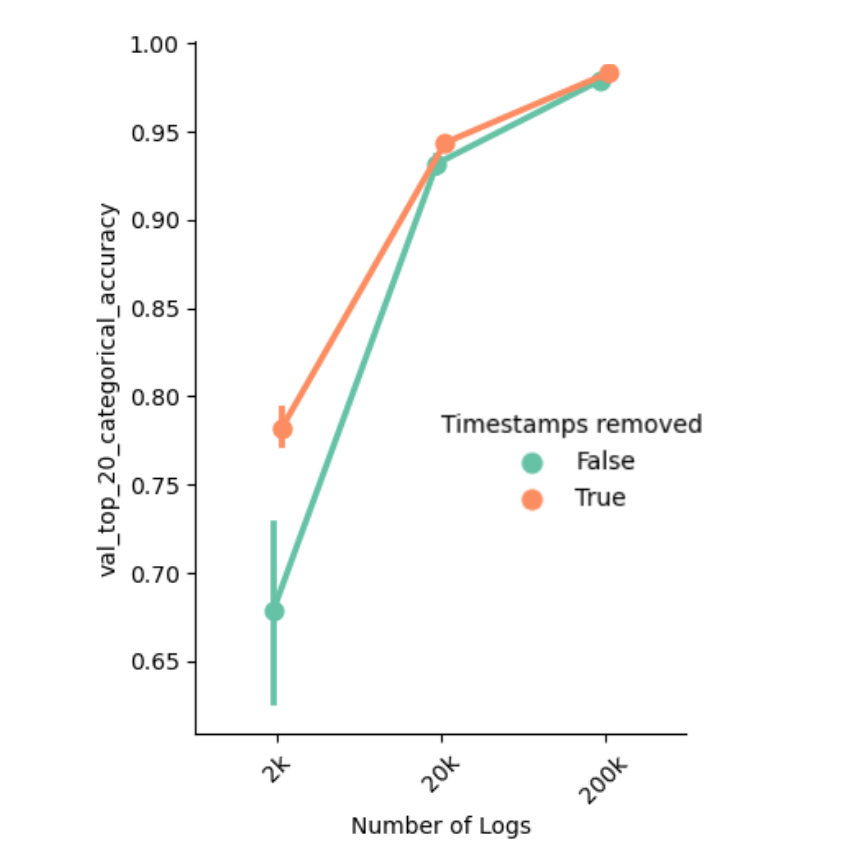
\includegraphics[keepaspectratio=true,scale=0.8]{figures/5_results/timestamps_comparison.png}
    \caption{Two line plots showing the prediction quality at different dataset sizes, with and without timestamps.}
    \label{fig:TimestampsComparison}
\end{figure}

When we look at the particular results for the biggest dataset, we can see that removing timestamps decreases variance of prediction quality across all fixed parameter templates. Finer granularity templates especially benefit from removing timestamps. 
\begin{figure}[H]
    \centering
    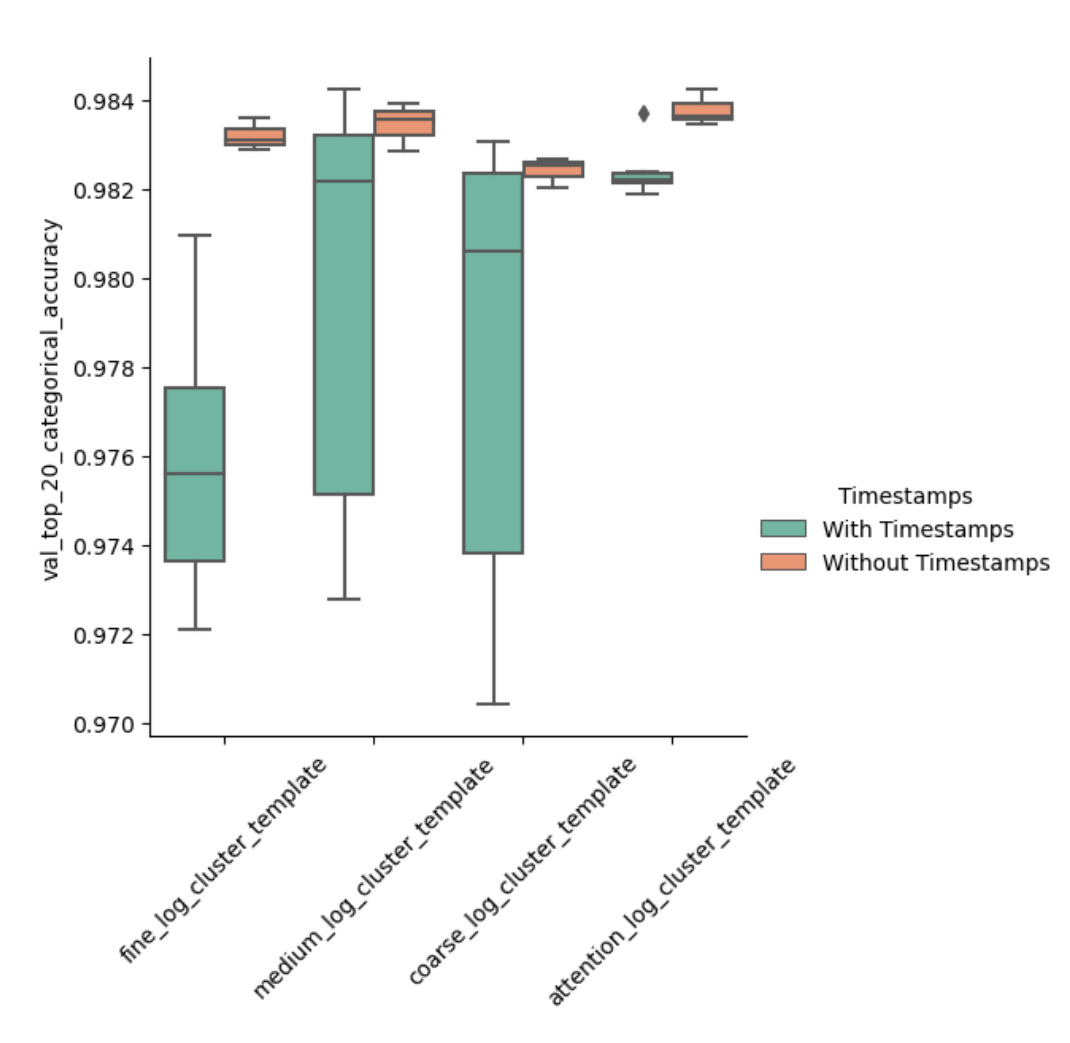
\includegraphics[keepaspectratio=true,scale=0.8]{figures/5_results/Timestamps_templates.png}
    \caption{The effect of timestamps on different levels of log template granularity and attention based selection. Dataset size 200k logs.}
    \label{fig:TimestampsTemplates}
\end{figure}

As can be seen in table \ref{tab:runtimes}, running the experiments with and without timestamps took approximately the same time for all dataset sizes. 
\begin{table}[htbp]
  \centering
  \begin{tabular}{ccc}
    \hline
    \textbf{Dataset Size} & \textbf{Runtime (With Timestamps)} & \textbf{Runtime (Without Timestamps)} \\
    \hline
    200k & 21.6 min & 22 min \\
    20k & 3.7 min & 3.7 min \\
    2k & 1.3 min & 1.3 min \\
        \hline

  \end{tabular}
    \caption{Runtime comparison with and without timestamps for different dataset sizes}
      \label{tab:runtimes}

\end{table}


\section{Individual Algorithms}
\label{sec:Results:Algos}
The attention mechanism, illustrated in figure \ref{fig:results:Algos}, delivered very good results, especially for Nulog and Spell, where it lead to the highest median accuracy of ~0.83 and ~0.84 respectively. Additionally, the data shows that not one type of granularity is best for each algorithm. Drain and Nulog benefited from more "finer" parameterization, while for Spell the "medium" settings lead to the best results, bar attention based selection. Overall, the results between the different log parsing algorithms are very similar at this dataset size. 

\begin{figure}[H]
     \centering
     \begin{subfigure}[b]{0.45\textwidth}
         \centering
        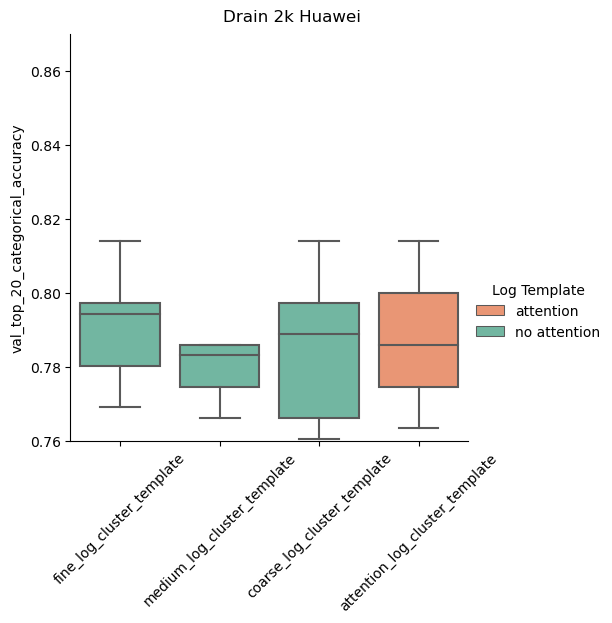
\includegraphics[keepaspectratio=true,scale=0.45]{figures/5_results/Drain_Huawei_2k.png}
         \caption{Drain}
         \label{fig:results:drain}
     \end{subfigure}
     \hfill
     \begin{subfigure}[b]{0.45\textwidth}
         \centering
        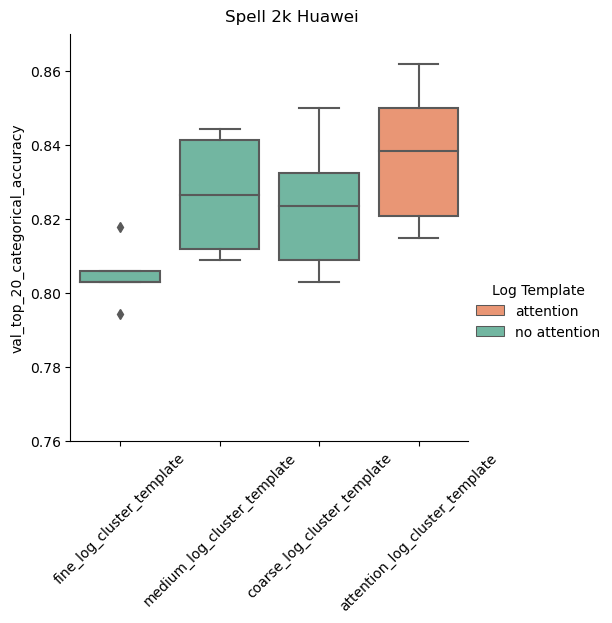
\includegraphics[keepaspectratio=true,scale=0.45]{figures/5_results/Spell_Huawei_2k.png}
         \caption{Spell}
         \label{fig:results:spell}
     \end{subfigure}
     \hfill
     \begin{subfigure}[b]{0.45\textwidth}
         \centering
        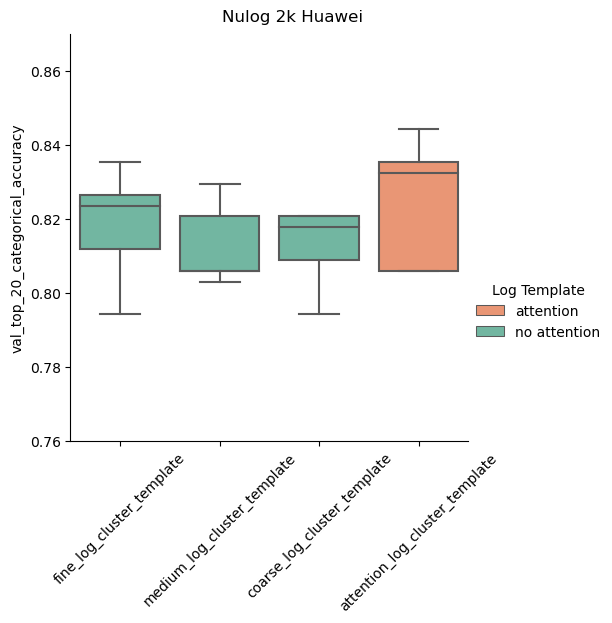
\includegraphics[keepaspectratio=true,scale=0.45]{figures/5_results/Nulog_Huawei_2k.png}
         \caption{Nulog}
         \label{results:nulog}
     \end{subfigure}
        \caption{Three plots comparing attention based selection to fixed parameter template baseline for Drain, Spell and Nulog. Dataset size 2000 logs. }
        \label{fig:results:Algos}
\end{figure}

With 2000 logs, the training time for our model is around 1.5 minutes for Spell and Drain and 3.5minutes for Nulog. Attention based selection had no impact on runtime at this dataset size. 

As can be seen in \ref{tab:log_parsers_comparison}, changing the parameters of the log parsers has great influence on the number of templates. Drain especially produces much more templates than the other two algorithms, which will become more obvious in the Thunderbird dataset.  

\begin{table}[htbp]
  \centering
  \begin{tabular}{ccccc}
    \hline
    \textbf{Parser} & \textbf{Fine} & \textbf{Medium} & \textbf{Coarse} & \textbf{Attention} \\
    \hline
    Drain & 198 & 174 & 154 & 526 \\
    Spell & 172 & 117 & 85 & 374 \\
    Nulog & 106 & 123 & 133 & 363 \\
    \hline
  \end{tabular}
  \caption{Effect of log parser parameterization on median number of generated log templates. Median values. Attention is the sum of the other three types of templates. Dataset size 2000 logs.}
  \label{tab:log_parsers_comparison}
\end{table}

\section{Combining multiple algorithms}
\label{sec:Results:Combination}
\subsection{All Algorithms}
When combining the templates generated by our log parsing algorithms Drain, Spell and Nulog and feeding it into the attention mechanism, the results are not as clear as with the individual parsers. While the difference in quality is lower, the attention mechanism still selected templates that led to the highest median accuracy of ~0.822. We observe that this value is slightly lower compared to using just Spell or Nulog. The runtime when using the templates generated by all log parsing algorithms is very similar compared to using only Nulog.

% Talked about runtime, template number is obvious?, quality. What else can I say here?

\begin{figure}[H]
    \centering
    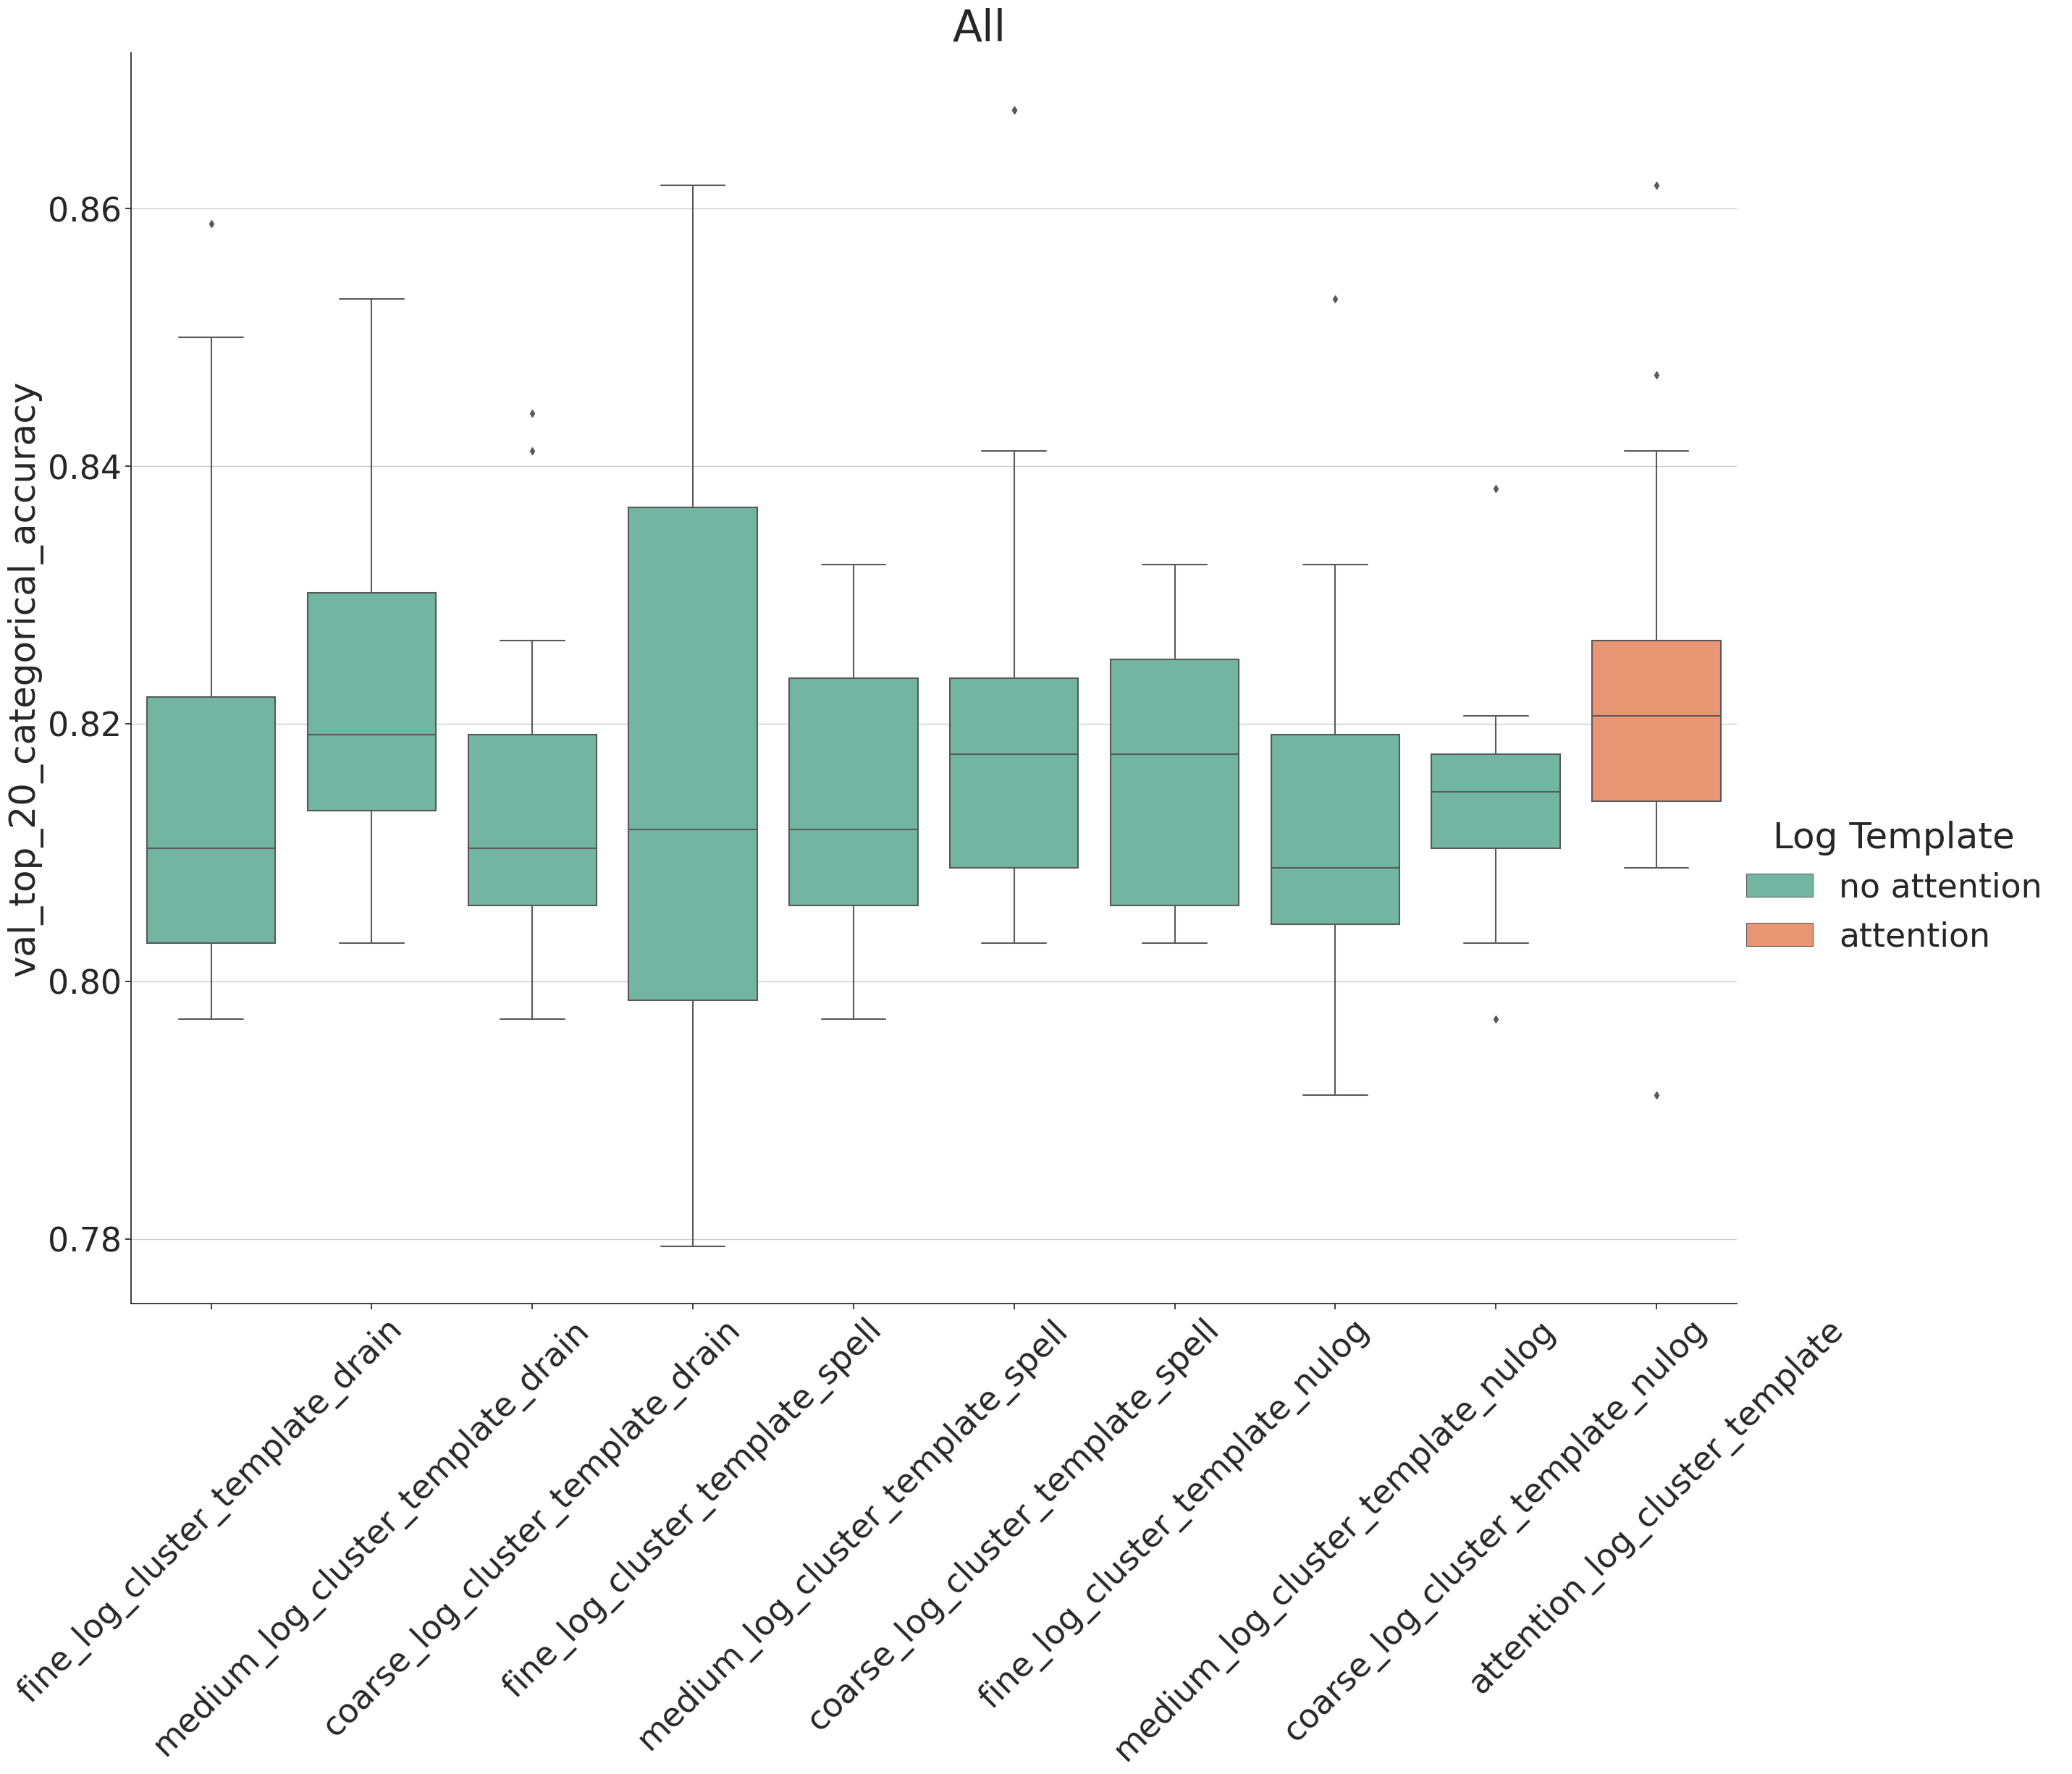
\includegraphics[keepaspectratio=true,scale=0.15]{figures/5_results/All_Huawei_2k.png}
    \caption{Attention based selection from nine log templates generated by three log parsers with three parameterizations. Dataset size 2000 logs.}
    \label{fig:all_together}
\end{figure}

\begin{table}[htbp]
  \centering

  \begin{tabular}{c c}
    \hline
    \textbf{Parser} & \textbf{Runtime} \\
    \hline
    Drain & 1.3 min \\
    Nulog & 4.1 min \\
    Spell & 1.2 min \\
    All & 4.2 min \\
    \hline
  \end{tabular}
    \caption{Runtime Comparison of Log Parsers}
  \label{tab:log_parsers_runtime}
\end{table}

\subsection{Combination of individual algorithms}
\label{sec:Results:Mixing}
We not only ran experiments using all log parsing algorithms at once, but also did tests with all possible combinations of two out three parsers. We can see in every figure, that no combination of log parsers resulted in a definite improvement compared to baseline as observed in the experiments using only a single log parsing algorithm. Interestingly, combining Drain and Spell led to better results than using all algorithms, as can be seen in figure \ref{fig:drain_spell}. The median accuracy with attention based selection in this experiment was ~0.835, compared to ~0.822 in figure \ref{fig:all_together}.

\begin{figure}[H]
    \centering
    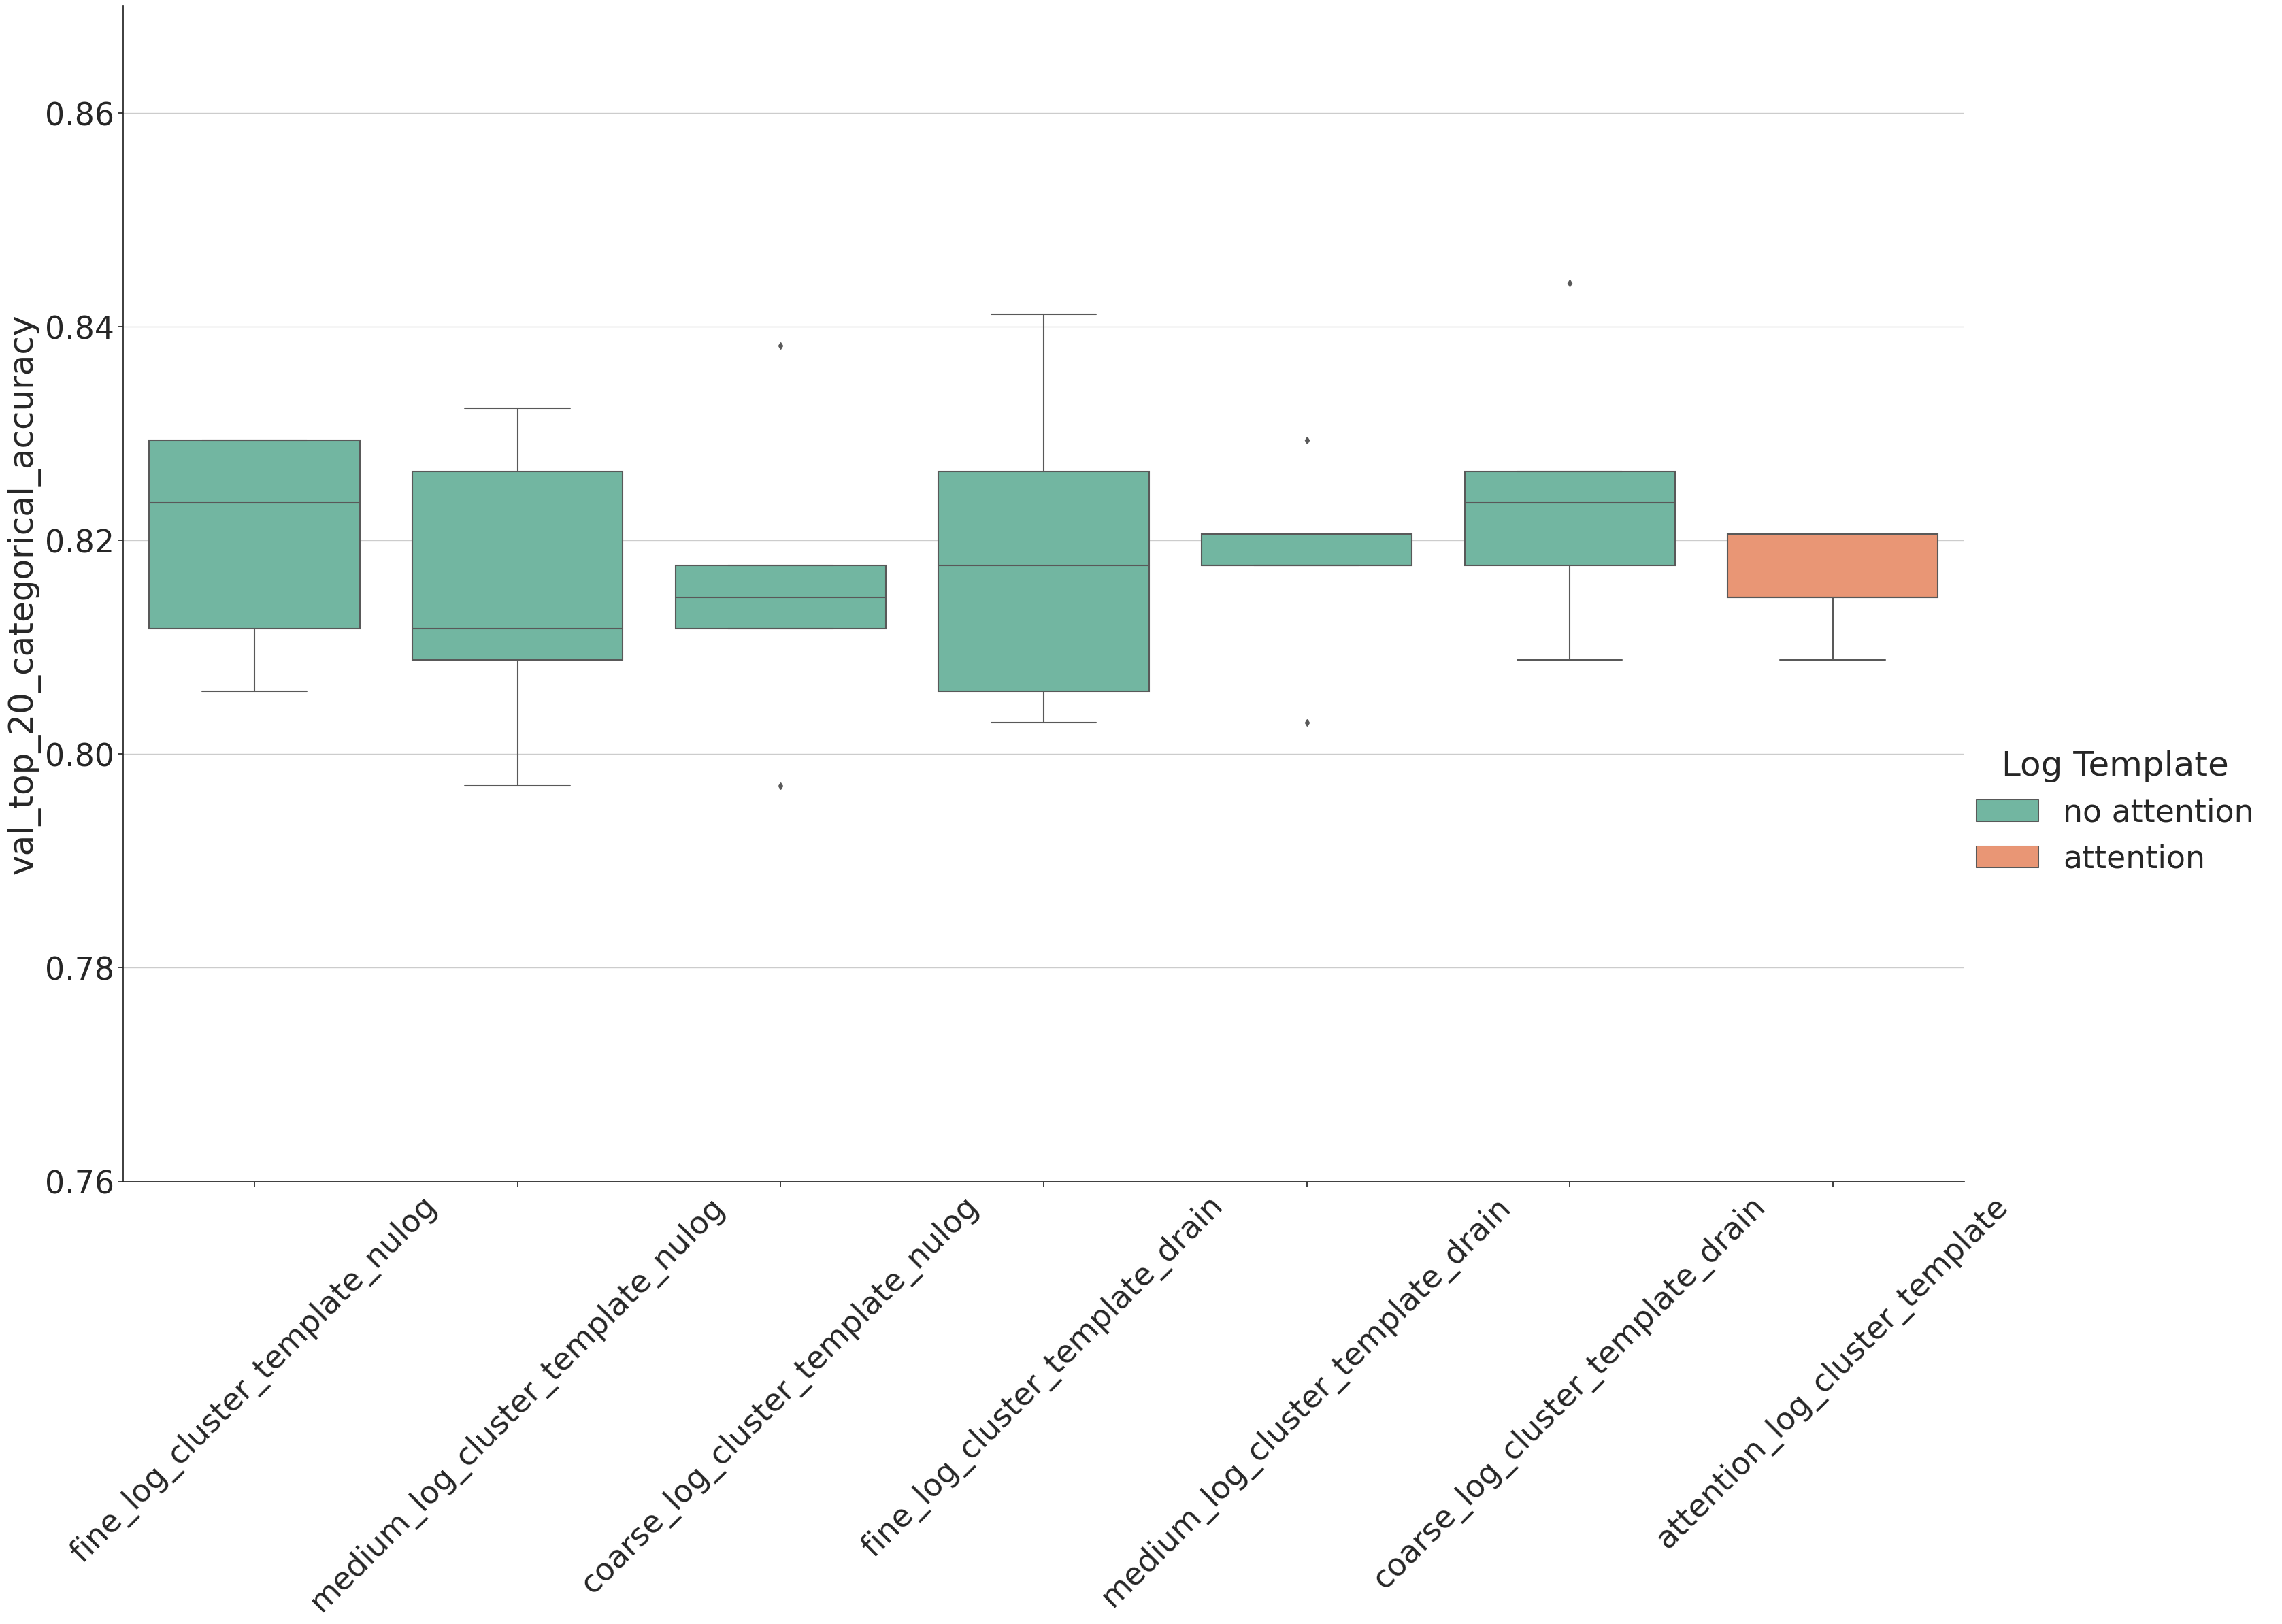
\includegraphics[keepaspectratio=true,scale=0.15]{figures/5_results/drain+nulog.png}
    \caption{Attention based selection from log templates generated Nulog and Drain. Dataset size 2000 logs.}
    \label{fig:drain_nulog}
\end{figure}

\begin{figure}[H]
    \centering
    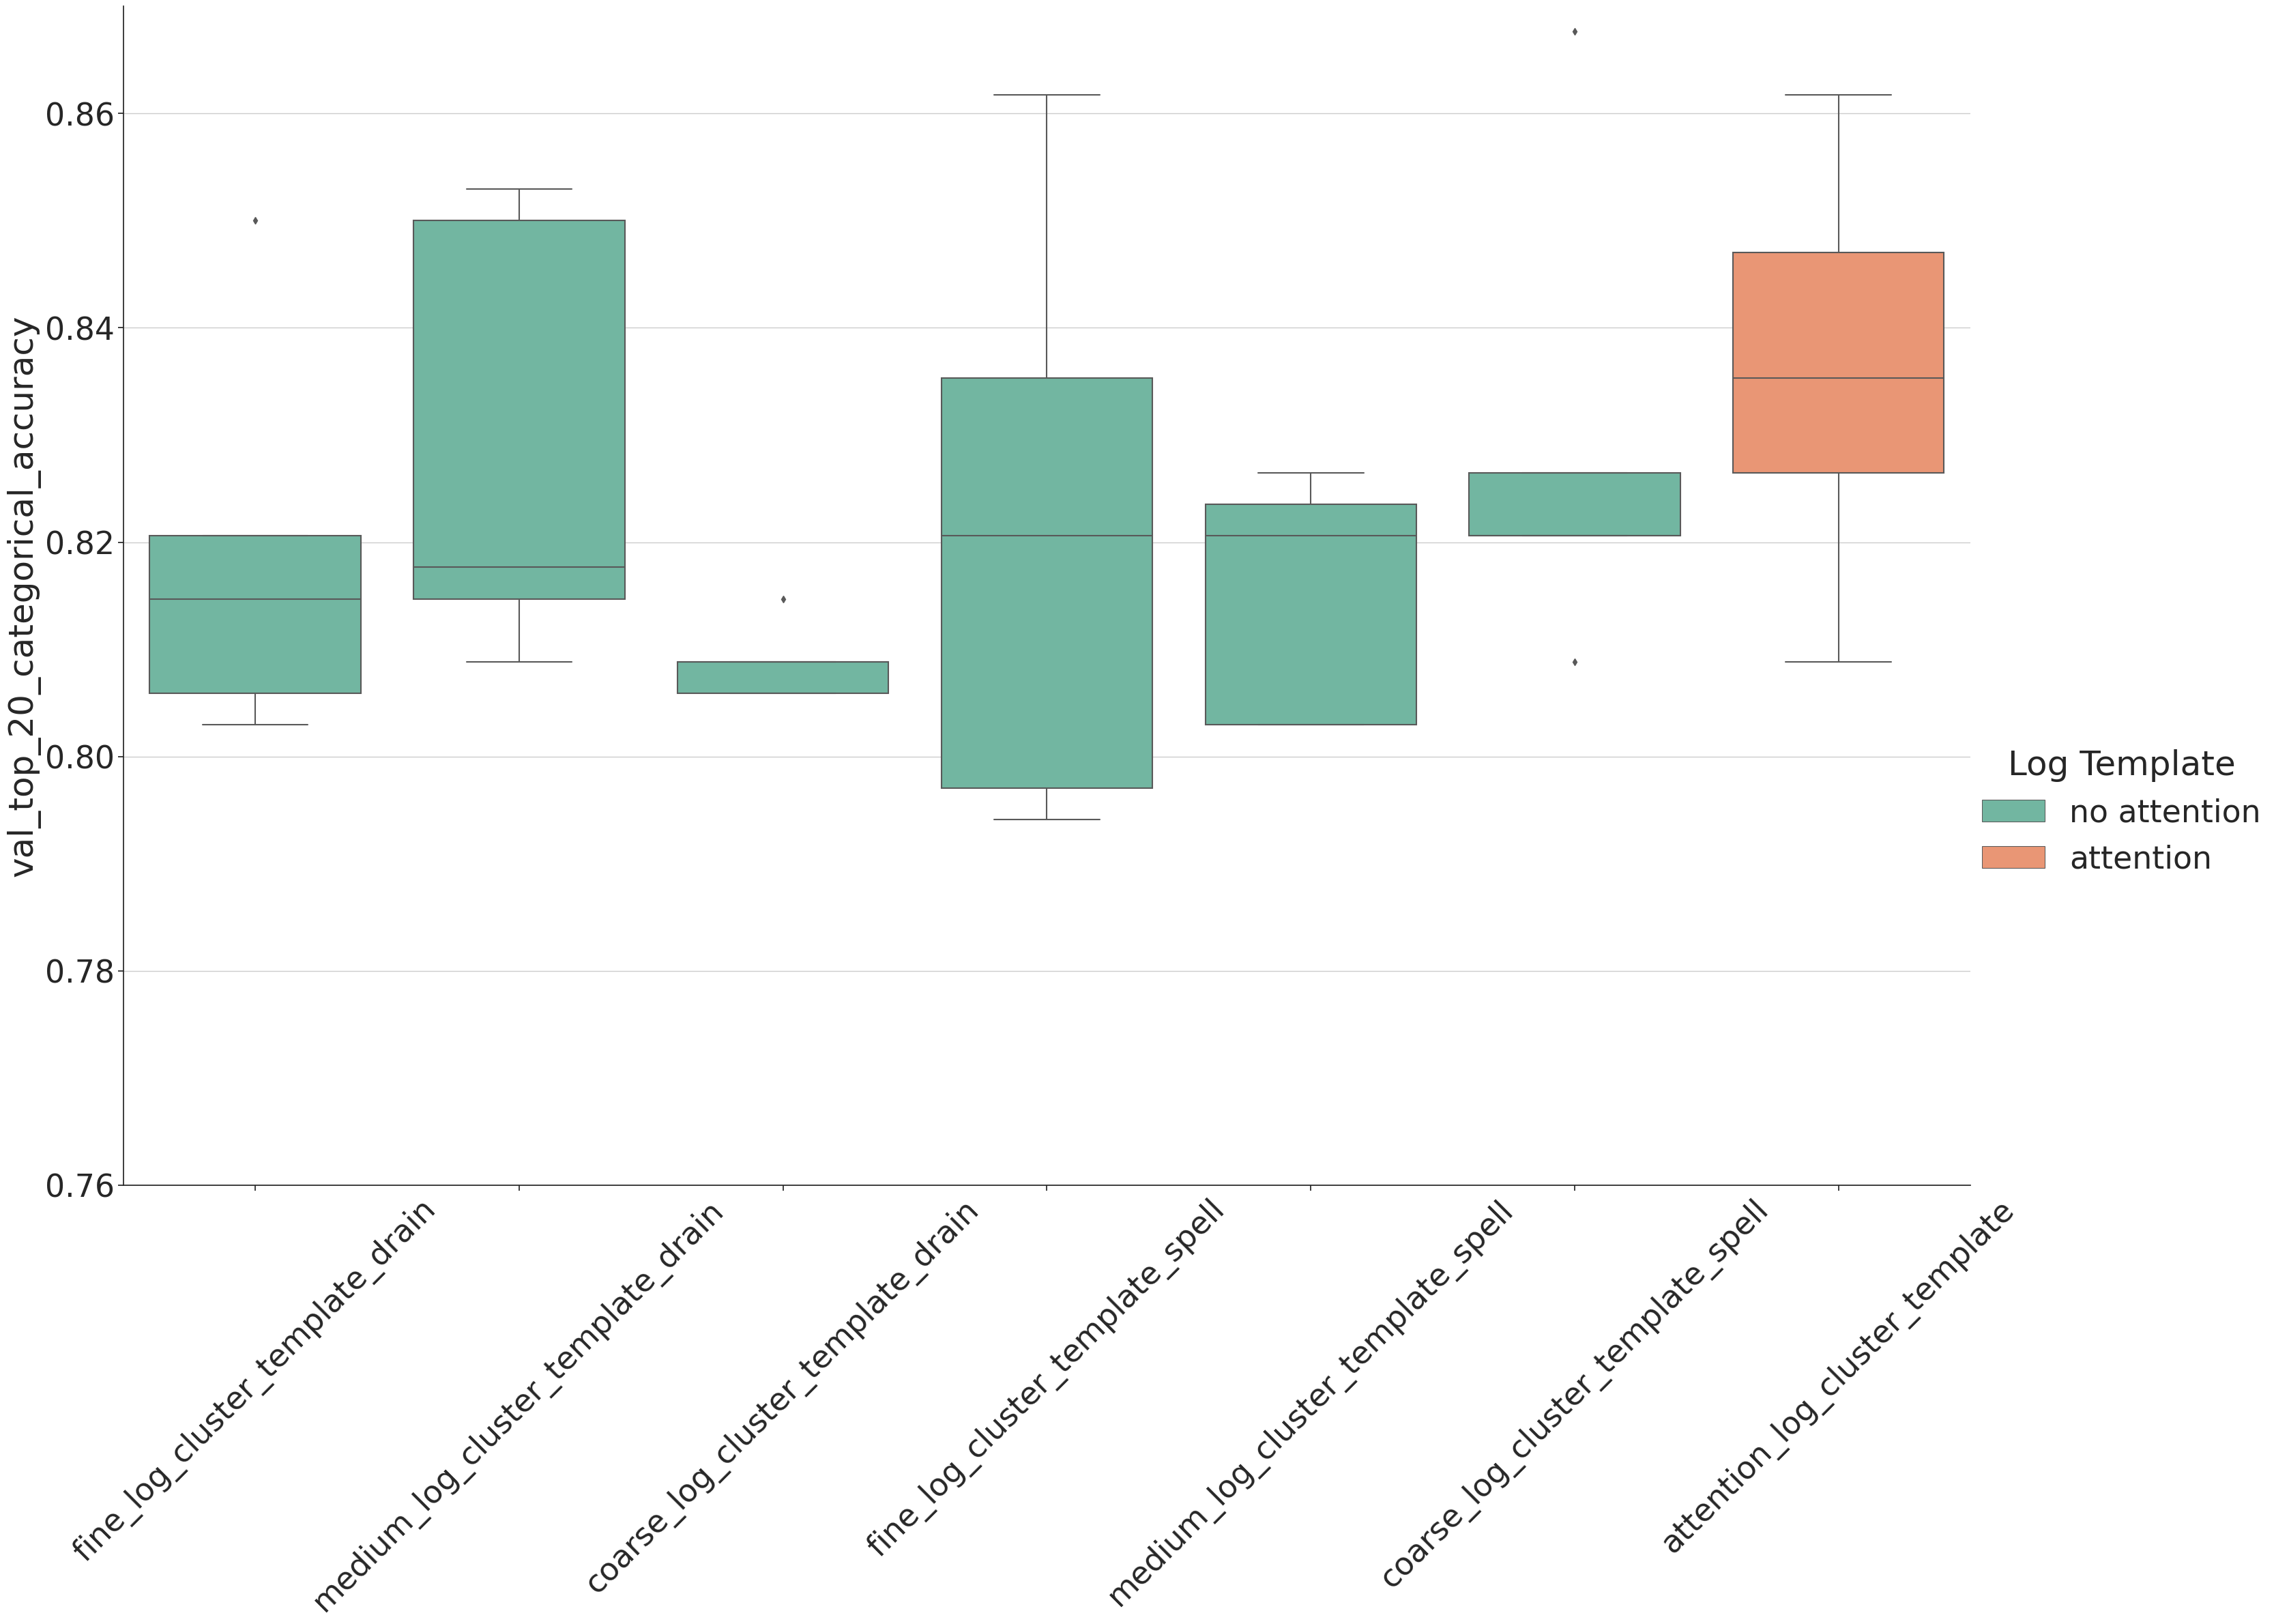
\includegraphics[keepaspectratio=true,scale=0.15]{figures/5_results/drain+spell.png}
    \caption{Attention based selection from log templates generated by Spell and Drain. Dataset size 2000 logs.}
    \label{fig:drain_spell}
\end{figure}

\begin{figure}[H]
    \centering
    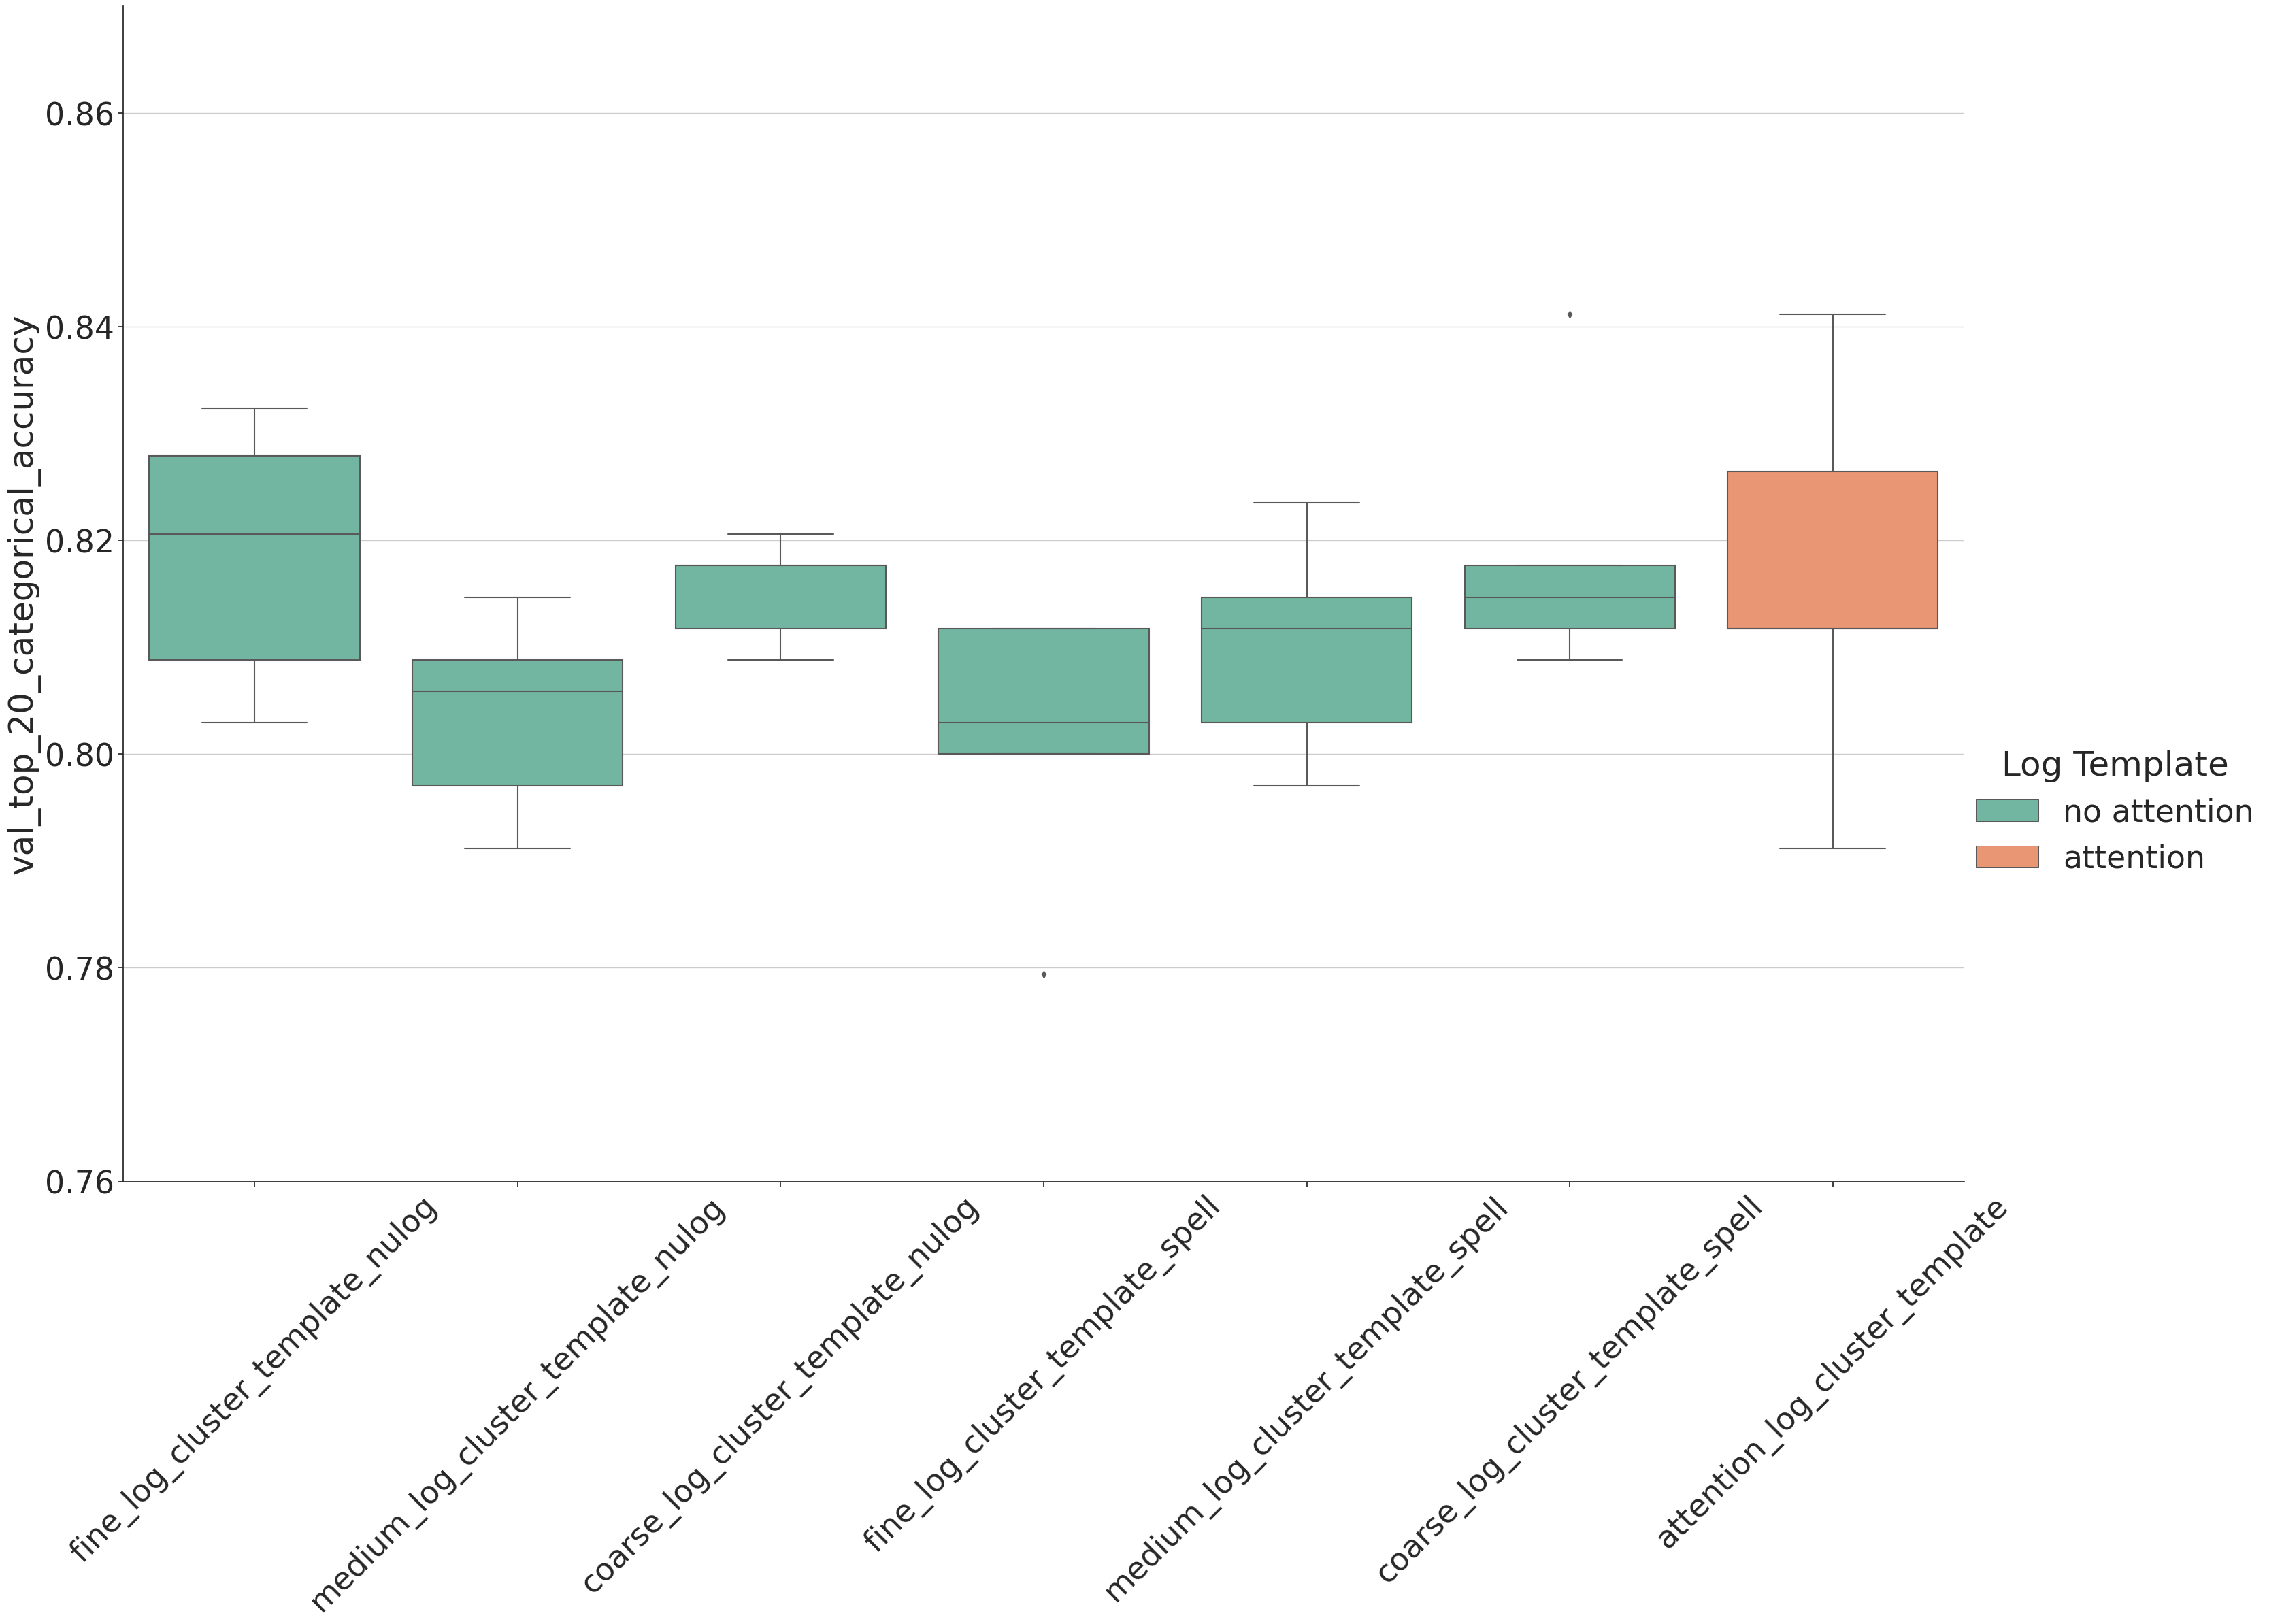
\includegraphics[keepaspectratio=true,scale=0.15]{figures/5_results/nulog+spell.png}
    \caption{Attention based selection from log templates generated by Nulog and Spell. Dataset size 2000 logs.}
    \label{fig:nulog_spell}
\end{figure}




\section{Other Datasets}
We repeated some of the experiments conducted with the original dataset with two other datasets, in particular, we evaluated the attention based selection of log templates generated by the individual algorithms and by a combination of all of them.

\subsection{HDFS}
On the HDFS dataset, we observed various differences compared to our experiments on the original logs. We can see in table \ref{tab:hdfs} that the number of templates generated by Drain is almost ten times higher compared to Nulog and Spell, which were much closer to each other for the original dataset. Furthermore, our model trained for much shorter than the 25 epochs that we set, which was also not the case with our previous experiment. The total runtime stayed very similar.  

\begin{table}[htbp]
  \centering
  \begin{tabular}{cccc}
    \hline
    \textbf{Parser} & \textbf{No. of Templates} & \textbf{Runtime} & \textbf{Epochs learned} \\
    \hline
    Drain & 441  & 1.8min & 9 \\
    Spell & 57   & 1.9min & 10 \\
    Nulog & 54  & 4.6min & 16 \\
    All & 553 & 4.7min & 16 \\
    \hline
  \end{tabular}
  \caption{Number of log templates, epochs learned and runtime for different log parsers. HDFS logs.}
  \label{tab:hdfs}
\end{table}

Figure \ref{fig:results:hdfs} shows the results for the individual log parsing algorithms, similar to figure \ref{fig:results:Algos}. We can see that the overall prediction quality is slightly worse and that Nulog performs best again. For all algorithms the templates selected by the attention mechanism do not lead to a better result, but in all cases the medium parameters delivered the best prediction quality. 

\begin{figure}[H]
     \centering
     \begin{subfigure}[b]{0.45\textwidth}
         \centering
        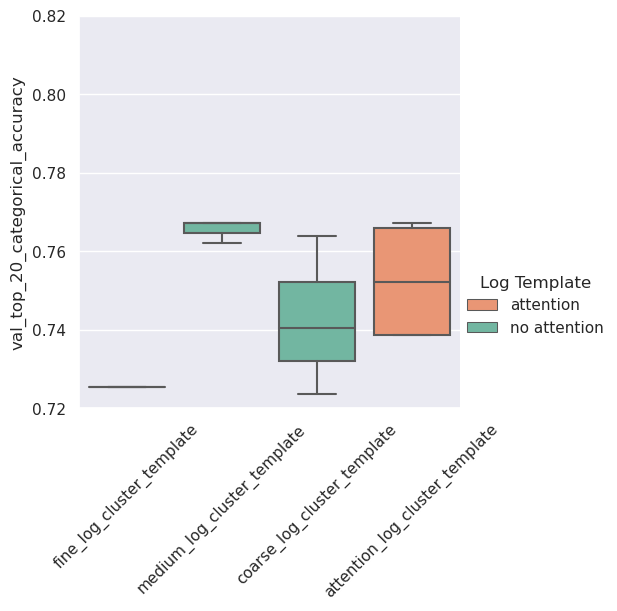
\includegraphics[keepaspectratio=true,scale=0.45]{figures/5_results/drain_hdfs.png}
         \caption{Drain}
         \label{fig:results:drain_hdfs}
     \end{subfigure}
     \hfill
     \begin{subfigure}[b]{0.45\textwidth}
         \centering
        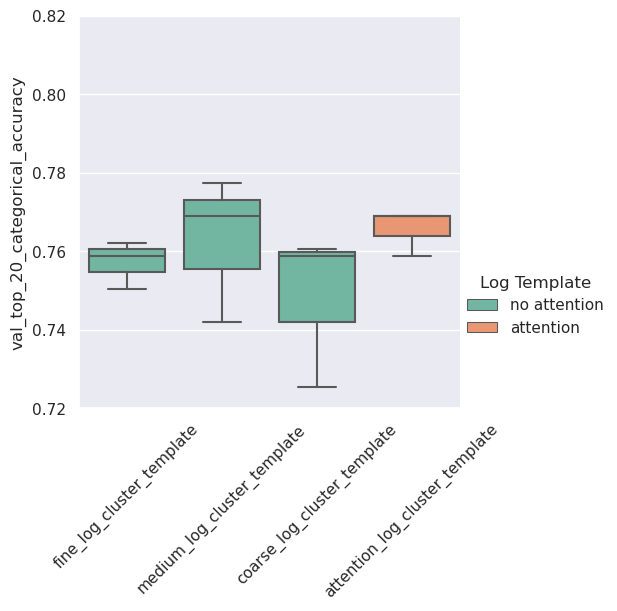
\includegraphics[keepaspectratio=true,scale=0.45]{figures/5_results/spell_hdfs.png}
         \caption{Spell}
         \label{fig:results:spell_hdfs}
     \end{subfigure}
     \hfill
     \begin{subfigure}[b]{0.45\textwidth}
         \centering
        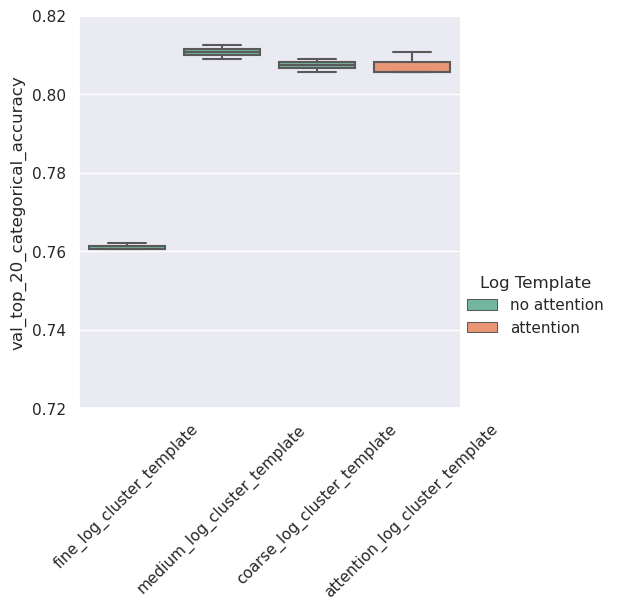
\includegraphics[keepaspectratio=true,scale=0.45]{figures/5_results/nulog_hdfs.png}
         \caption{Nulog}
         \label{results:nulog_hdfs}
     \end{subfigure}
        \caption{Three plots comparing attention based selection to fixed parameter template baseline for Drain, Spell and Nulog. Dataset size 2000 logs. }
        \label{fig:results:hdfs}
\end{figure}

Figure \ref{fig:average_hdfs} shows the average prediction quality of all individual log parsers. We can see here that  attention selected templates lead to a higher median accuracy, but that this improvement is very small. 

\begin{figure}[H]
    \centering
    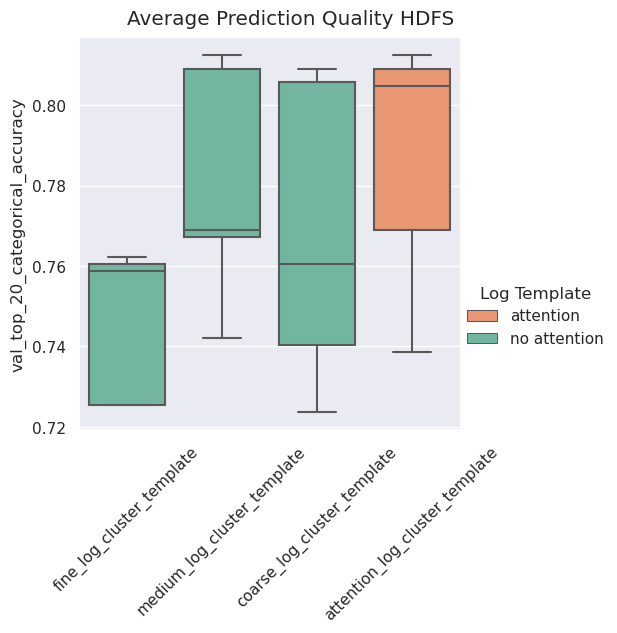
\includegraphics[keepaspectratio=true,scale=0.6]{figures/5_results/average_hdfs.png}
    \caption{Average prediction quality over all log parsing algorithms. Dataset size 2000 logs.}
    \label{fig:average_hdfs}
\end{figure}

When feeding all the templates from all our parsers into the attention mechanism, we observe that the attention results are very good and on par with the Nulog results, but are not the best overall as can be seen in figure \ref{fig:all_hdfs}.
\begin{figure}[H]
    \centering
    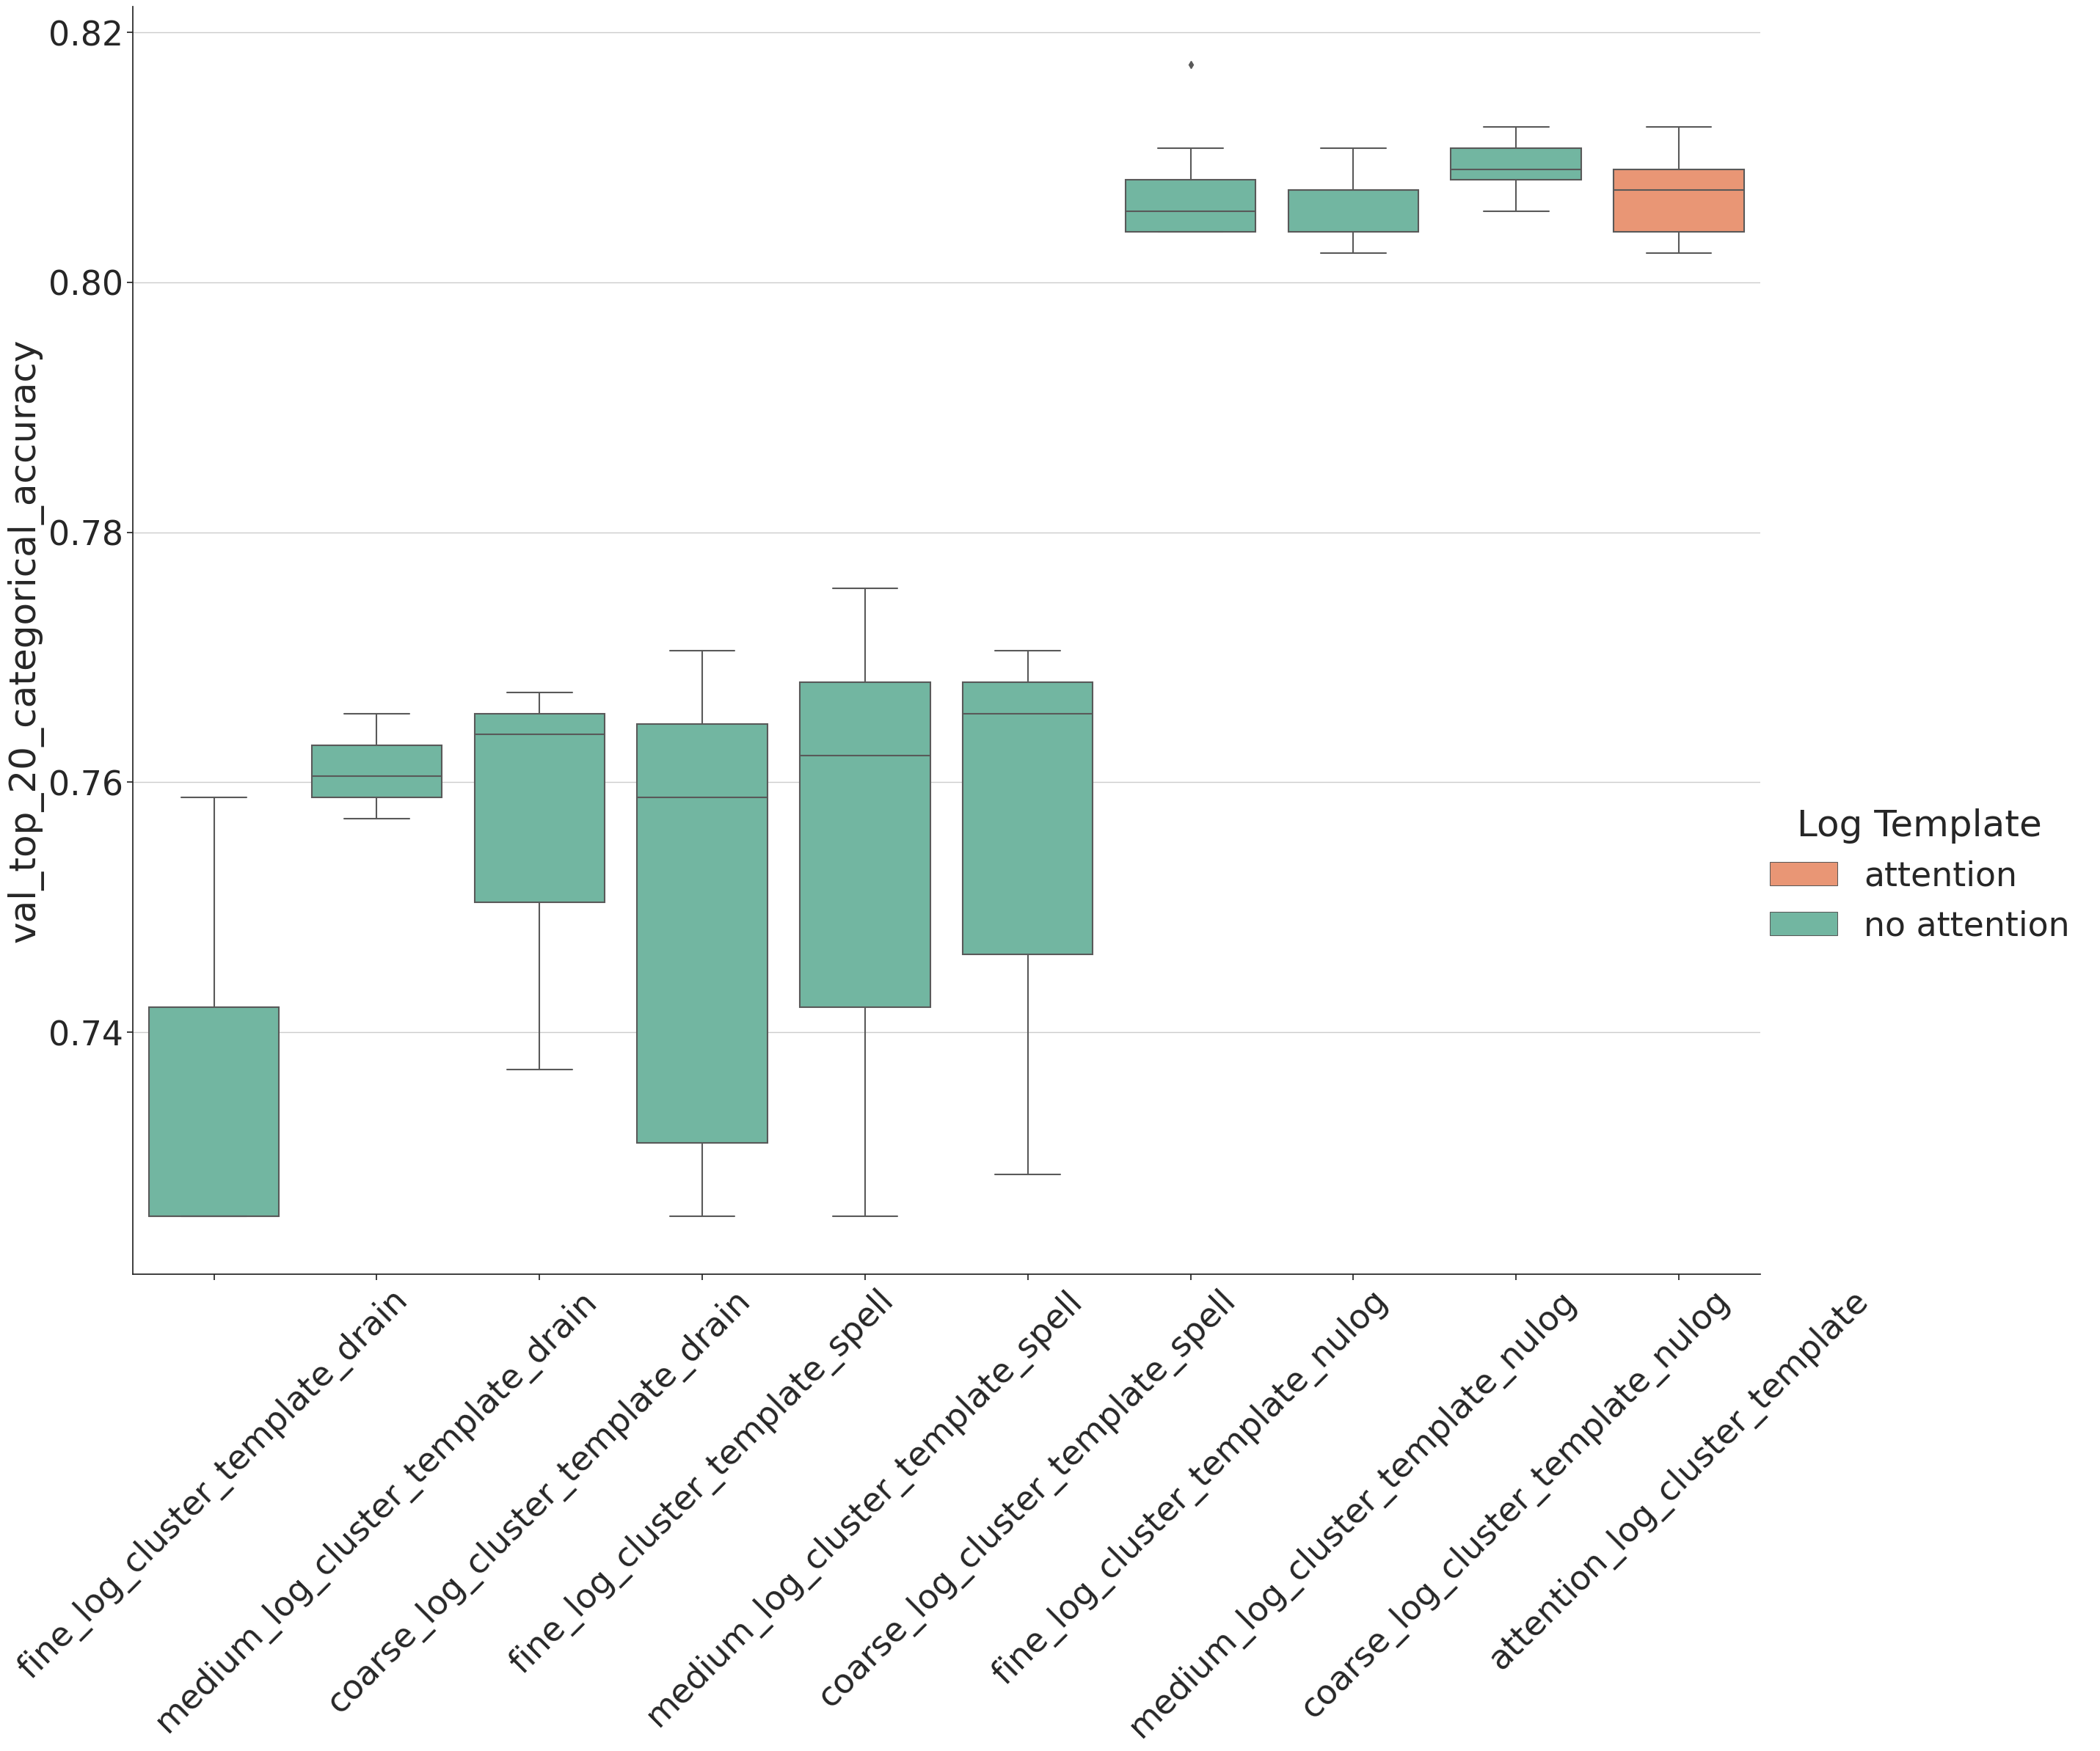
\includegraphics[keepaspectratio=true,scale=0.2]{figures/5_results/all_hdfs.png}
    \caption{Attention based selection from nine log templates generated by three log parsers with three parameterizations. Dataset size 2000 logs.}
    \label{fig:all_hdfs}
\end{figure}

Motivated by our earlier results that showed that using Drain and Spell performed better than combining all three algorithms [Figure \ref{fig:drain_spell}], we ran another experiment just with Nulog and Spell, because drain performed badly on this dataset. Contrary to the earlier experiment, we saw no improvement. 

\begin{figure}[H]
    \centering
    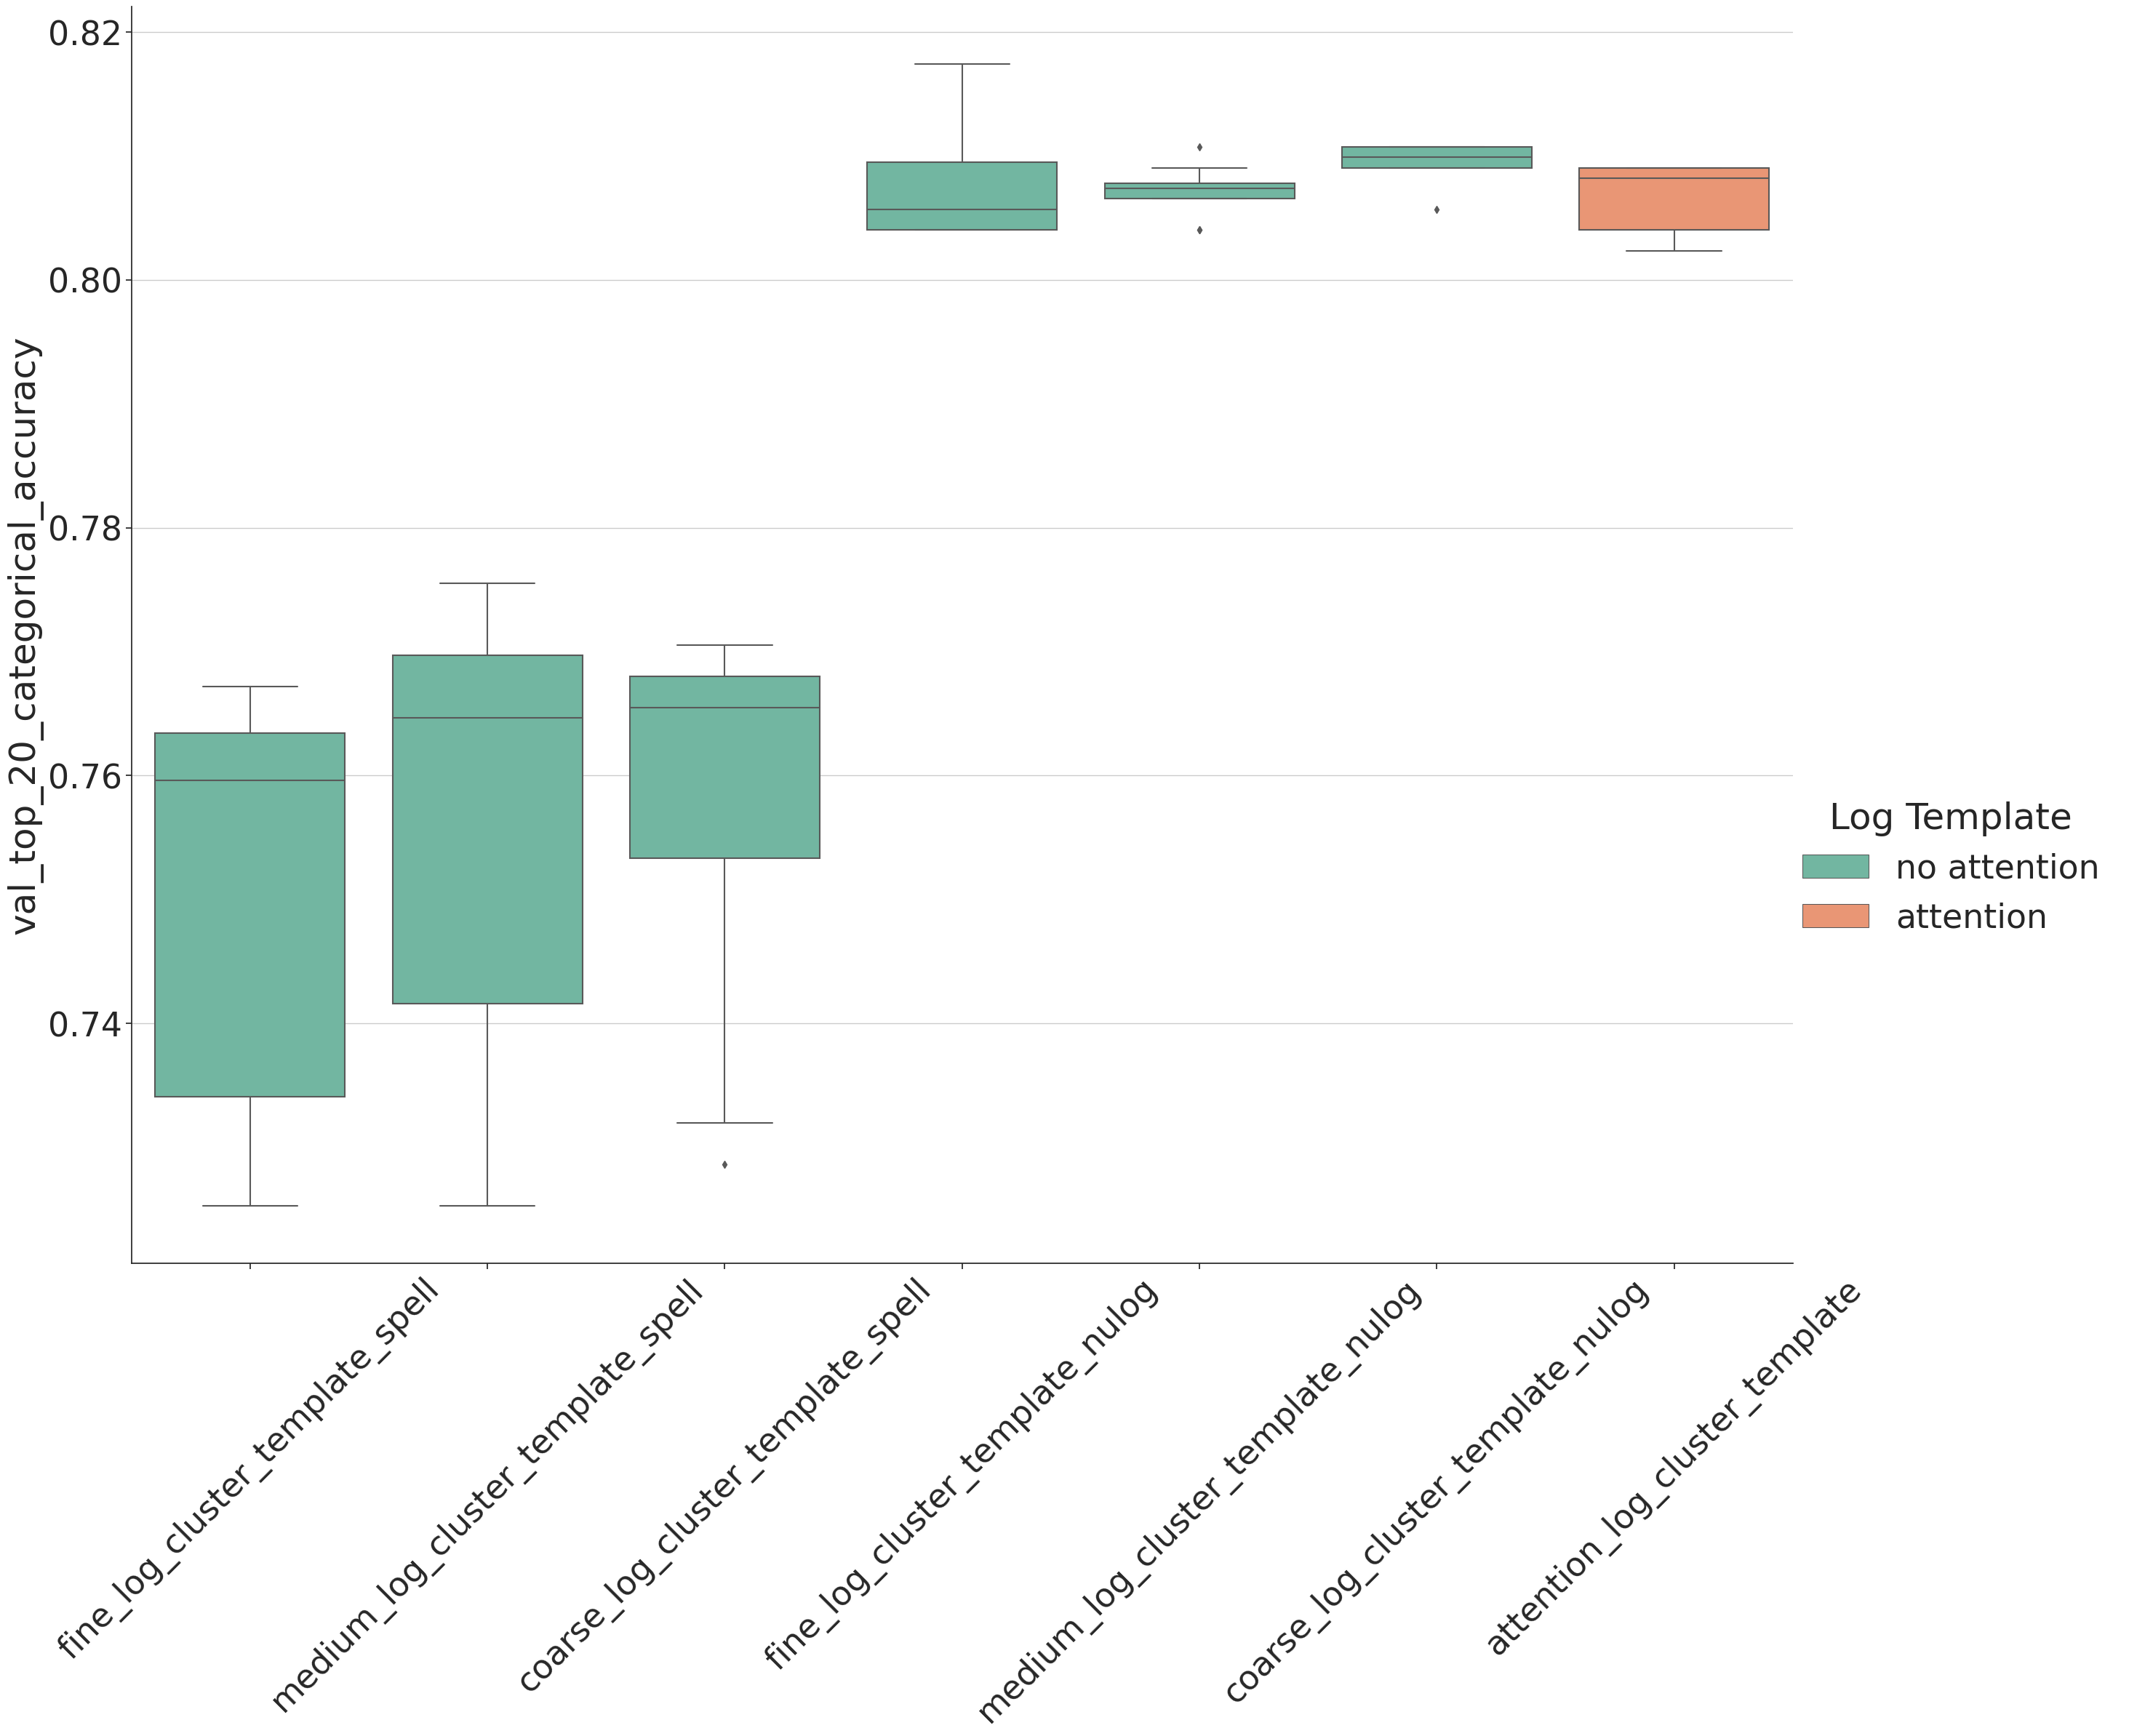
\includegraphics[keepaspectratio=true,scale=0.2]{figures/5_results/spell_nulog_hdfs.png}
    \caption{Attention based selection from six log templates generated by Spell and Nulog with three parameterizations. Dataset size 2000 logs.}
    \label{fig:spell_nulog_hdfs}
\end{figure}

\subsection{Thunderbird}
The results from our Thunderbird experiments differed the most from our original dataset. Drain produced by far the most templates, while the number of templates was generally already much higher than for the other datasets. Using drain templates alone also led to the highest experiment runtime, longer even than when using the combination of all templates. During our Drain and Spell experiments, the model also stopped learning very early and did not improve its validation accuracy beyond the initial value. 

\begin{table}[htbp]
  \centering
  \begin{tabular}{cccc}
    \hline
    \textbf{Parser} & \textbf{No. of Templates} & \textbf{Runtime} & \textbf{Epochs learned} \\
    \hline
    Drain & 2661  & 12.1min & 6 \\
    Spell & 456   & 1.2min & 7 \\
    Nulog & 397  & 4.3min & 14 \\
    All & 3402 & 4.2min & 14 \\
    \hline
  \end{tabular}
  \caption{Number of log templates, epochs learned and runtime for different log parsers. Thunderbird logs. }
  \label{tab:thunderbird}
\end{table}

We can see in figure \ref{fig:all_tbird} several identical results for the prediction quality with no variance and generally very close, low values. 

\begin{figure}[H]
    \centering
    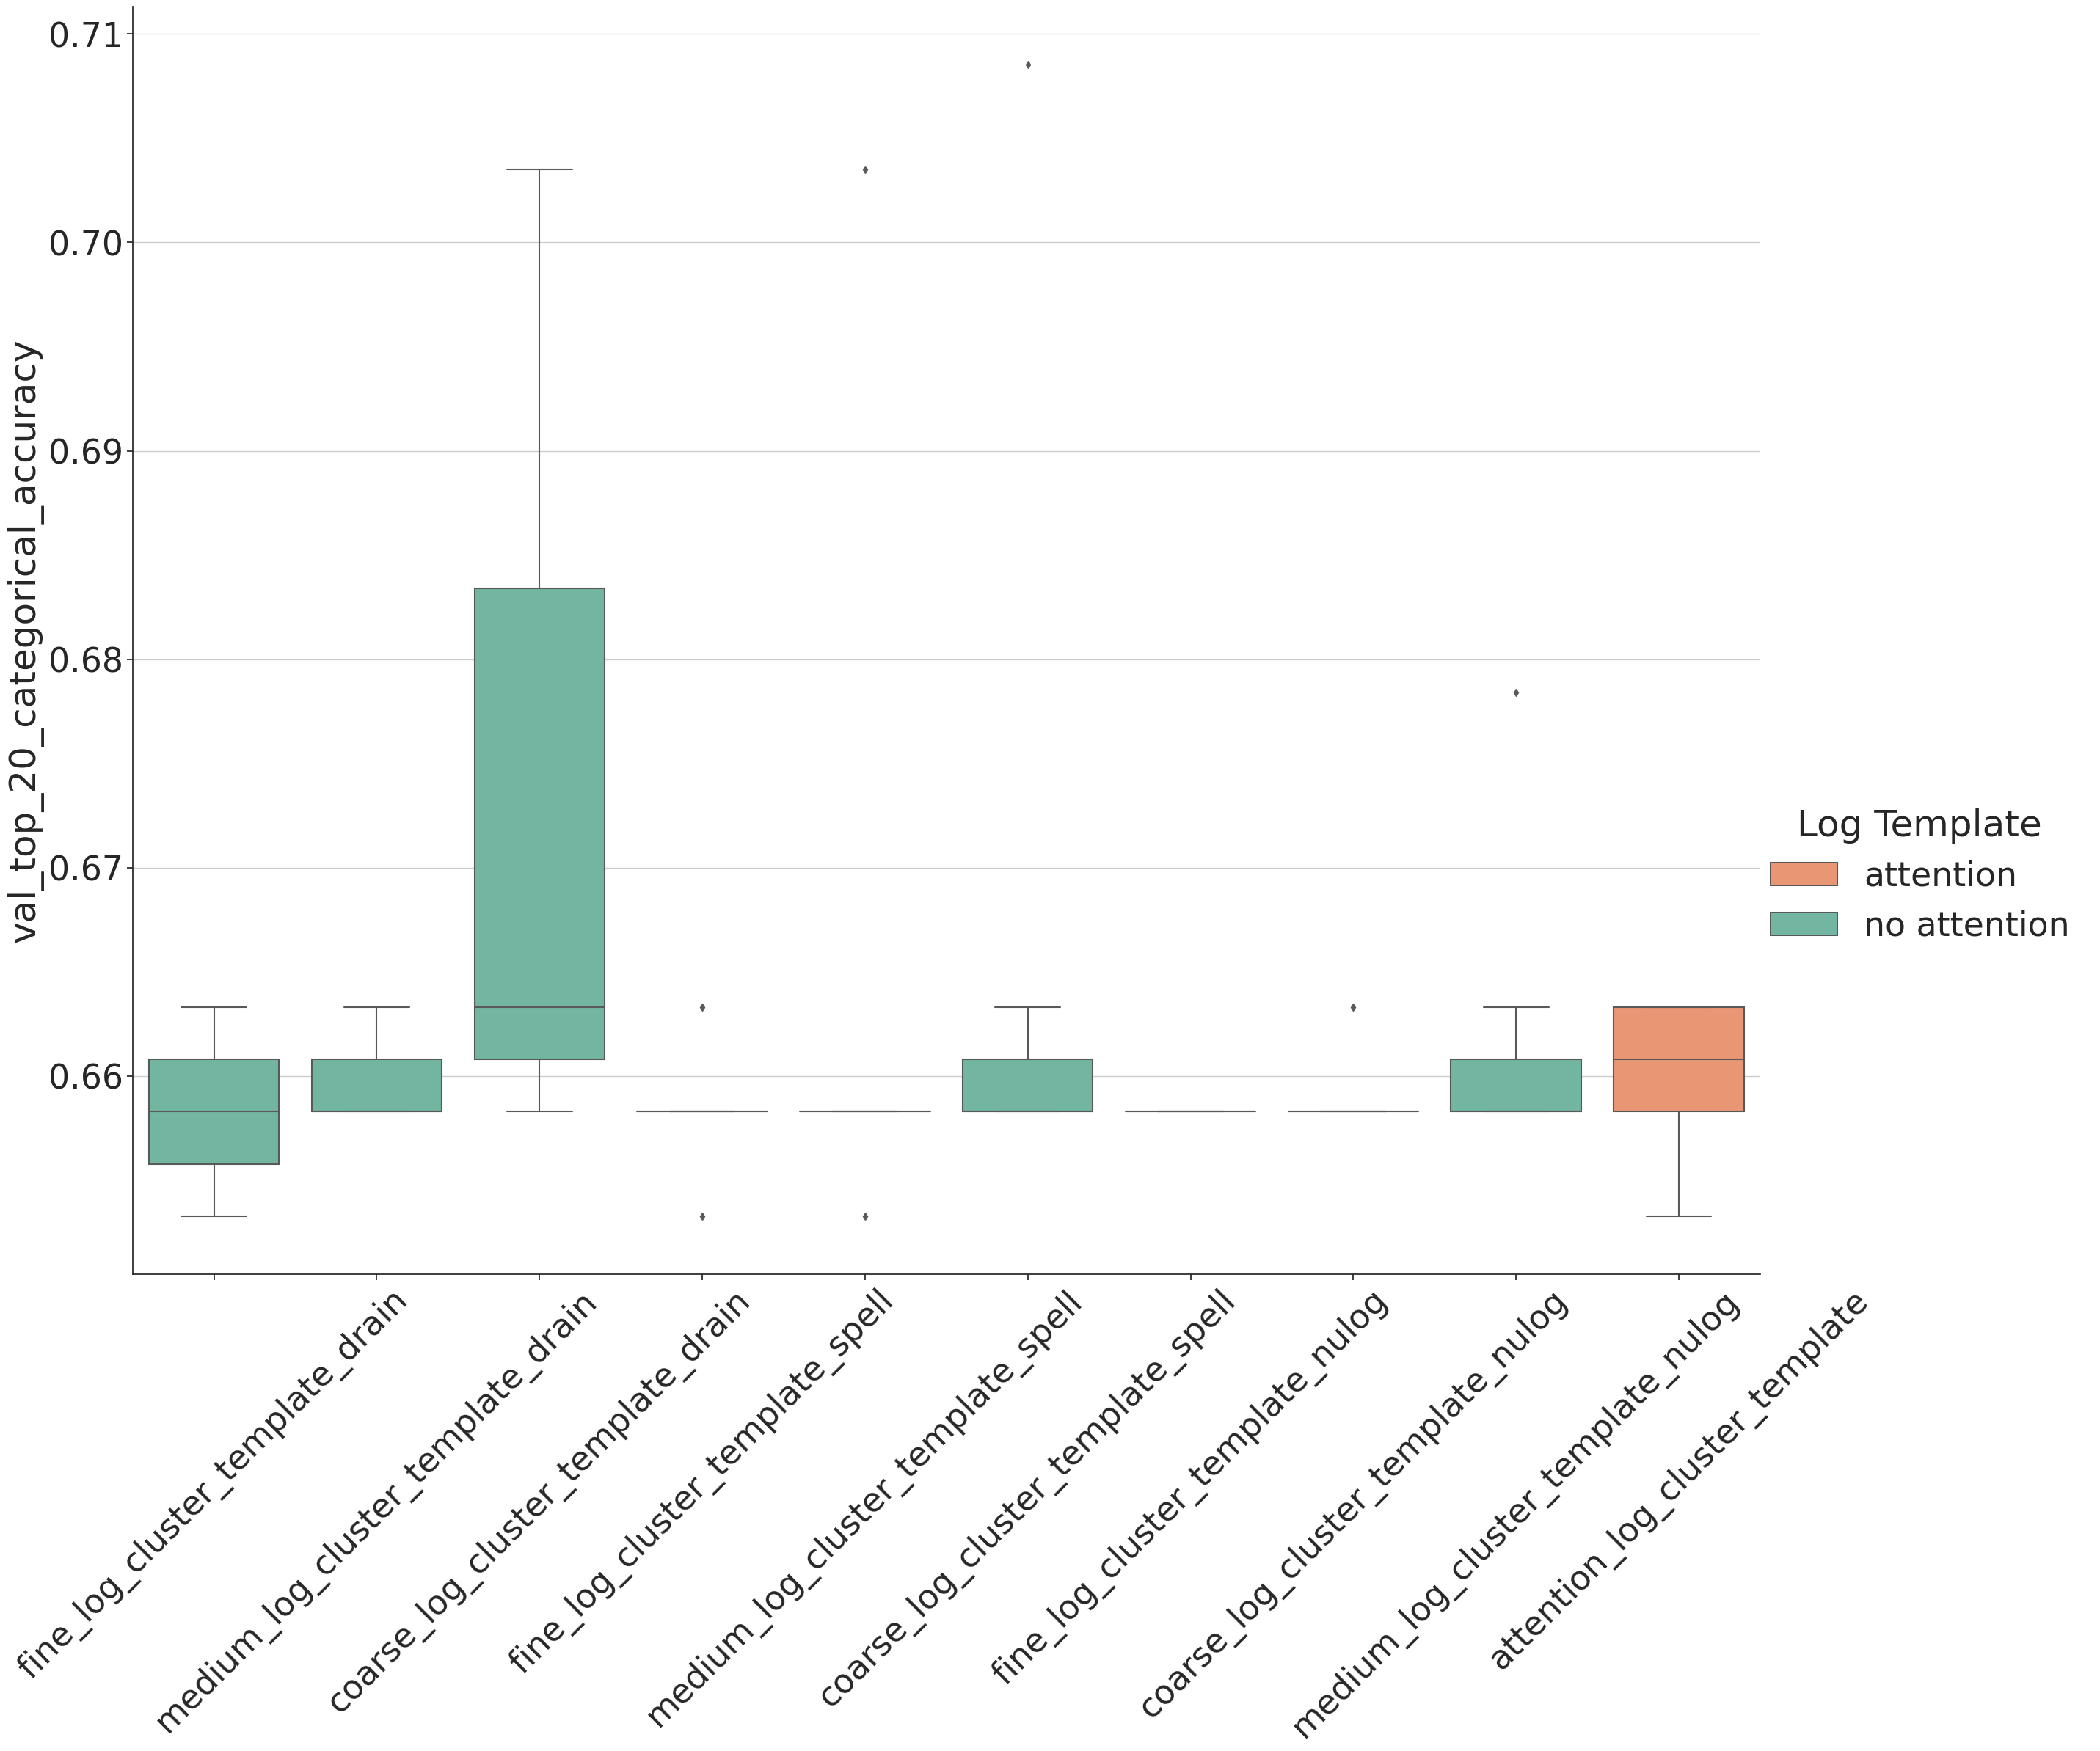
\includegraphics[keepaspectratio=true,scale=0.2]{figures/5_results/all_tbird.png}
    \caption{Attention based selection from nine log templates generated by three log parsers with three parameterizations. Dataset size 2000 logs.}
    \label{fig:all_tbird}
\end{figure}
\chapter{Discussion}
\label{ch:Discussion}
In chapter \ref{ch:Results} we presented the detailed results for each of our conducted experiments. This section focuses on some high-level observations that we made during the course of this project. 

\section{Generalizability}
\subsection{Other Algorithms}
We found that the attention mechanism can be used with other log parsing algorithms as can be seen in figure \ref{fig:results:Algos}. The data also shows that the overall quality of the prediction is dependent on the used parser and that using a more suitable parser for the task leads to better prediction results. In the prior thesis that developed this approach \cite{witterauf2021domainml}, we could see a strong improvement of attention based selection over baseline, but the author only presented the top five categorical accuracy, while we are more interested in the top 20 prediction quality. The author also observed this kind of improvement for a much larger dataset, which we could replicate in our timestamp experiments where we also used the same size dataset as can be seen in figure \ref{fig:TimestampsTemplates}. We hypothesise that when using larger amounts of data, we would observe a similar improvement for Nulog and Spell on the original dataset. At our smaller dataset size of 2000 logs, the attention mechanism still performed well and could be used to increase the robustness of the parsing step towards changes in the log structure, especially since there is no runtime penalty for using it. \\

Our experiments showed that when combining more templates from different parsers and feeding more information into the attention mechanism, the selected templates do not lead to a significantly better prediction quality, as can be seen in figure \ref{fig:all_together}. One possible explanation is that there is a sweet spot for the numbers of templates to offer as a selection that might also depend on the dataset size. So offering nine different templates per log at 2000 total logs might be too much. Another reason could be the overall similarity of the different log templates so that the attention mechanism does not learn clearly some most important template for the prediction task. \\



\subsection{Other datasets}
When performing our experiments on the other two datasets, Thunderbird and HDFS, we could not observe an additional benefit of using attention. For Thunderbird, our baseline results were already much worse than the other datasets'. We try to explain these results in this section.\\

One specialty of our original dataset is its large amount of distinct attributes, compared to the other two datasets. While we look at eight different attributes for our next attribute prediction in the Huawei logs, we only use one attribute as prediction target with Thunderbird logs and three with HDFS logs. This lack of structure in the underlying data could explain some part of the bad results. Our original dataset also contained different types of logs: application logs, error logs, system logs, while HDFS and Thunderbird are more homogeneous, each in their own way. \\

The parameters that were set up for the different log parsing algorithms were tuned on the original dataset and have just been copied for our new datasets. It is possible that they are highly unsuited for this type of logs and that the results would look different with other parameters. \\

As mentioned throughout this work: the sizes of the dataset could've also played a large role in the results. As our overall quality and also the difference between attention based selection and baseline decreased when we went from the full Huawei log dataset, it is possible that scaling up the experiments to bigger dataset sizes could lead to better results. 

\section{Timestamps}
Before we conducted our timestamp experiments, our hypothesis was that timestamps act as noise at large dataset sizes and removing them should improve the prediction accuracy, while at smaller dataset sizes they should be beneficial to learning and contain important information for the prediction. We wanted to find the point where timestamps turn from helpful to hindering. We also predicted that log templates with finer granularity should especially benefit from the removal of timestamps. \\

Our experiments then showed it is true that fine log templates benefited the most from the removal, as in these templates the time stamps often remain intact or get parsed as below:
\begin{verbatim}
    23 06 11 17:33:25 -> * * 11 17 33 25
\end{verbatim}

This is in contrast to the more coarse templates, which might look like this, depending on the parser and specific parameters:
\begin{verbatim}
    23 06 11 17:33:25 -> * * * * * 25 
\end{verbatim}

Furthermore, we observed that the robustness of our prediction greatly increased, similar to the effect of using attention based selection. One possible explanation could be, that the attention mechanism assigned very low importance to the timestamp part of the log templates and that our removal of the timestamps has a similar effect to this ranking. \\ 

On the other hand, it was at the dataset size of 2000 logs that the removal of timestamps had the most positive and significant impact on prediction quality. We believe that the reason for this is that at a lower dataset size, the relative share of timestamps compared to the rest of the log messages is higher, while also not containing helpful information for the prediction part and acting as the kind of noise we hypothesised for large datasets. \\

We only conducted our timestamp experiments on a single dataset and with one algorithm, but we believe that these results would translate to other datasets and algorithms as well and that the removal of timestamps should be incorporated into the log analysis workflow. 

%% LaTeX2e class for student theses
%% sections/conclusion.tex
%% 
%% Karlsruhe Institute of Technology
%% Institute for Program Structures and Data Organization
%% Chair for Software Design and Quality (SDQ)
%%
%% Dr.-Ing. Erik Burger
%% burger@kit.edu
%%
%% Version 1.3.5, 2020-06-26

\chapter{Conclusion}
\label{ch:Conclusion}
At the beginning of the project we assumed that when combining multiple log parsing algorithms and feeding the generated templates into an attention mechanism, this would lead to improved results compared to only using a single algorithm. \\

We started off by reproducing the original results and then extending the existing codebase to handle multiple different log parsing algorithms and datasets. The original results were improved even more by using other log parsing algorithms that performed better. Parallel to this, we came up with our timestamp hypothesis and conducted the corresponding experiments. We showed that the removal of timestamps has a beneficiary effect on prediction quality across all dataset sizes, but smaller datasets benefited the most.  Thus, we recommend to incorporate timestamp removal as a preprocessing step in the log analysis workflow. \\

After evaluating different log parser combinations and datasets, we can not conclude that this attention based selection method is effective at improving prediction quality. 


\section{Further research}
We conducted the majority of our experiments only on rather small datasets. Future research could repeat these experiments on much larger and more realistically sized datasets and check whether the originally observed positive effects would materialize again. Since we had good results with one dataset, it would be interesting to research what made the experiments successful on this dataset and whether it has some specific properties that made this method work, if the reason for our negative results was not the dataset size. \\

Additionally, we recommend further experiments to solidify our timestamp results and establish the removal of timestamps as a standard preprocessing step. 
\chapter{Acknowledgements}
\label{ch:achnowledgements}
I would like to thank Prof. Klemens Böhm for giving me the opportunity to work on this interesting topic. \\

Special thanks have to go out to my supervisor Pawel Bielski. He taught me a lot about the research process, invested a lot of time in me and this project and pushed me to give my best. I think him for all the meetings, the valuable feedback on my presentations, his patience and tenacity.  \\


I also want to use this chance to thank my friends Jan, Max, Ismar and Yoki for their open ears and their support during all the years of studying at KIT. Without you guys the time at university would not have been half as fun. 


%% --------------------
%% |   Bibliography   |
%% --------------------

%% Add entry to the table of contents for the bibliography
\printbibliography[heading=bibintoc]

%% ----------------
%% |   Appendix   |
%% ----------------
%\appendix
%%% LaTeX2e class for student theses
%% sections/apendix.tex
%% 
%% Karlsruhe Institute of Technology
%% Institute for Program Structures and Data Organization
%% Chair for Software Design and Quality (SDQ)
%%
%% Dr.-Ing. Erik Burger
%% burger@kit.edu
%%
%% Version 1.3.5, 2020-06-26

\iflanguage{english}
{\chapter{Appendix}}    % english style
{\chapter{Anhang}}      % german style
\label{chap:appendix}

\section{Thevenin Model}
\label{sec:TheveninFormula}
This section gives an in-depth look into the mathematical computation that is needed to obtain the formulas of the Thevenin Model. If we simplify our current input, we can even describe the voltage in distinct phases during charging.
\subsection{General Case}
\begin{figure}[H]
    \centering
    \includegraphics[keepaspectratio=true,scale=0.7]{figures/8_appendix/theveninCircuit.png}
    \caption{Illustration of the equivalent circuit of the Thevenin model \cite{plett2018batterybootcamp}.}
    \label{fig:circuitThev}
\end{figure}
The overall current is dependent on the two individual currents, flowing through the resistor $R_1$ and capacitor $C_1$: 
\begin{equation} \label{eq:thev1}
i_{R_1}(t) + i_{C_1}(t) = i(t).
\end{equation}
Since 
\begin{equation} \label{eq:thev2}
C = \frac{Q}{U} \Rightarrow i(t) = C \cdot \frac{d \, U(t)}{d \, t} 
\end{equation}
and 
\begin{equation} \label{eq:thev3}
R_1 = \frac{U_1}{i_{R_1}} \Leftrightarrow U_1 = R_1 \cdot i_{R_1},
\end{equation}
we get: 
\begin{equation} \label{eq:thev4}
i_{C_1}(t) = C_1 \cdot R_1 \cdot \frac{d \, i_{R_1}(t)}{d t}.
\end{equation}

When we now insert equation \ref{eq:thev4} in equation \ref{eq:thev1} (using $\tau_1 = R_1 C_1$), we obtain the differential equation
\begin{equation} \label{eq:thev5}
i_{R_1}(t) + \tau_1 \cdot \frac{d \, i_{R_1}(t)}{d t} = i(t),
\end{equation}
whose solution is
\begin{equation} \label{eq:thev6}
i_{R_1}(t) = i_{R_1}(t_0) \cdot \exp{\bigg(-\frac{t-t_0}{\tau_1}\bigg)} + \frac{1}{\tau_1} \cdot \int_{t_0}^{t} \exp{\bigg(-\frac{t-t'}{\tau_1}\bigg)} \cdot i(t') \; d t'.
\end{equation}

The voltage of this electrical circuit is influenced by the OCV, the two resistors $R_0$ and $R_1$ as well as the capacitor $C_1$. Therefore, it can be described with:
\begin{equation} \label{eq:thev7}
v(t) = \text{OCV}(z(t)) - R_1 \cdot i_{R_1}(t) - R_0 \cdot i(t).
\end{equation}

With the SOC being:

\begin{equation} \label{eq:thev8}
z(t) = z(t_0) - \frac{1}{Q} \cdot \int_{t_0}^{t} i(t') \; d t'.
\end{equation}

If we insert equation \ref{eq:thev6} into equation \ref{eq:thev7} we get:
\begin{equation} \label{eq:thev9}
v(t) = \text{OCV}(z(t)) - R_1 \cdot i_{R_1}(t_0) \cdot \exp{\bigg(-\frac{t-t_0}{\tau_1}\bigg)} - \frac{1}{C_1} \cdot \int_{t_0}^{t} \exp{\bigg(-\frac{t-t'}{\tau_1}\bigg)} \cdot i(t') \; d t' - R_0 \cdot i(t).
\end{equation}

\subsection{Special Case}
If we only consider current profiles of rectangular shape, we can describe the different voltage formulas separately. For illustration we use a rectangular discharge profile defined as follows:

\begin{equation} \label{eq:thev10}
i(t) =
\left\{
	\begin{array}{ll}
		0  & \mbox{if } t < 0 \\
		-i_0 & \mbox{if } 0 \leq t \leq t_p \\
		0 & \mbox{if } t > t_p
	\end{array}
\right.
\end{equation}

We can describe the different voltages separately using multiple case distinctions:

\paragraph{$t < 0$}
\begin{equation} \label{eq:thev11}
\begin{gathered} 
v(t) = \text{OCV}(z_0) \\
z_0 = z(0) 
\end{gathered}
\end{equation}

\paragraph{$0 \leq t \leq t_p$}
\begin{equation} \label{eq:thev12}
\begin{gathered} 
v(t) = \text{OCV}(z(t)) + i_0 \cdot R_1 \cdot \bigg(1 - \exp{\bigg(-\frac{t}{\tau_1}\bigg)}\bigg) + R_0 \cdot i_0 \\
z(t) = z(0) + \frac{i_0}{Q} \cdot t
\end{gathered}
\end{equation}

\paragraph{$t > t_p$}
\begin{equation} \label{eq:thev13}
\begin{gathered} 
v(t)  = \text{OCV}(z_p) + i_0 \cdot R_1 \cdot \exp{\bigg(-\frac{t}{\tau_1}\bigg)} \cdot
\bigg(\bigg(\exp{\bigg(\frac{t_p}{\tau_1}\bigg)} - 1\bigg)\bigg) \\
z_p = z(0) + \frac{i_0}{Q} \cdot t_p 
\end{gathered}
\end{equation}



\end{document}
